% USC Dissertation/Thesis LaTeX Template
% Edited by Ruda Zhang, 2020-10-08.
% -----------------------------------------------------------------------------
%	PACKAGES AND DOCUMENT CONFIGURATION
%-----------------------------------------------------------------------------

% Use `report` class with `USCthesis` package (style file) by Brian P. Gerkey
% Font size should be 11 or 12 points for regular paragraph text.
\documentclass[letterpaper,12pt]{report}
\usepackage[dissertation]{USCthesis}

% Packages required by `USCthesis.sty`.
\usepackage{hyperref}
\usepackage{setspace}
\usepackage{tabularx}

% Line spacing and margins in compliance with USC graduate school guidelines.
\usepackage[margin=1in,footskip=.5in]{geometry}
\doublespacing

% Optional packages: mathematical fonts and symbols
% You may comment this section out if you don't need them.
\usepackage{mathptmx} % set font to Times Roman
\usepackage[OT1]{fontenc} % font encoding for xelatex
\usepackage{mathtools}
\usepackage{amsmath, amssymb, amsthm}

% Optional packages: graphics
\usepackage{calrsfs} % For other scripts
\DeclareMathAlphabet{\pazocal}{OMS}{zplm}{m}{n}
\SetMathAlphabet\pazocal{bold}{OMS}{zplm}{bx}{n}
\usepackage{listings} % For code
\usepackage{caption} % For captioning tables?
\usepackage{graphicx}
\usepackage{tikz}
\usetikzlibrary{arrows,shapes,positioning} % For graphics in Permutation Statistics paper
\usetikzlibrary{decorations.pathreplacing} % For graphics in Spinning Switches
\usepackage{chessfss} % For chess pieces: \rook.
\usepackage[subnum]{cases} % For labeling parts of cases in Permutation Statistics paper
\usepackage[shortlabels]{enumitem} % For numbering enum
\usepackage{multirow} % For \multirow in Permutation Statistics paper
\newcommand{\n}[1]{\multicolumn{1}{|c|}{#1}} % For Permutation Statistics tables
\newcommand{\nW}[2]{\tikz[remember picture,anchor=base, baseline,inner xsep=0pt]{\node[box](#2){\vphantom{$\int$}$\underline{#1}$};}}
\newcommand{\nS}[1]{\tikz[remember picture,anchor=base, baseline,inner xsep=0pt]{\node[box](#1){\vphantom{$\int$}\textvisiblespace};}}
\newcommand{\bm}{\boldsymbol}
\pgfmathsetmacro{\myinnersep}{2}% inner sep in mm
\tikzset{
box/.style={
    inner sep=0,%
    outer sep=0,%
    minimum height=5mm,%
    align=center}
}

% You can use the "demo" option while editing to avoid compiling figures.
% \usepackage[demo]{graphicx}
% You can add absolute paths as well.
\graphicspath{{./}{../}{figures/}{../figures/}}

% Optional packages: bibliography with BibLaTeX.
% Comment this section out if you prefer BibTeX.
\usepackage[
    style=nature,
    sorting=none,
    isbn=false,
    url=false,
    doi=true,
    eprint=false,
    date=year,
    maxnames=6,
    minnames=6
]{biblatex}
\AtEveryBibitem{\clearfield{eventtitle}}
\AtEveryCitekey{\clearfield{eventtitle}}
\AtEveryBibitem{\clearfield{pagetotal}}
\AtEveryCitekey{\clearfield{pagetotal}}
\addbibresource{references.bib}

% Filler text for formatting. Comment these lines out for real writing.
\usepackage[english]{babel}
\usepackage{csquotes}
\usepackage{blindtext}

\newtheorem{theorem}{Theorem}[section]
\newtheorem{note}[theorem]{Note}
\newtheorem{definition}[theorem]{Definition}
\newtheorem{conjecture}[theorem]{Conjecture}
\newtheorem{openquestion}[theorem]{Open Question}
\newtheorem{lemma}[theorem]{Lemma}
\newtheorem{corollary}[theorem]{Corollary}
\newtheorem{example}[theorem]{Example}
\newtheorem{proposition}[theorem]{Proposition}
\newtheorem{claim}[theorem]{Claim}
\newtheorem*{problem}{\$100 Problem}
\newtheorem*{answer}{\$100 Answer}
\begin{document}

%-----------------------------------------------------------------------------
%	TITLE PAGE
%-----------------------------------------------------------------------------

% Volume name could be added as option, e.g. `[Volume I]`.
\title{\textbf{\Large{Permutations, Statistics, and Switches}}}

\author{Peter Kagey}

% Committee list is only shown in `proposal` layout.
\committee{S.~Assaf & (Chair)\\*
           R.~Arratia\\*
           D.~Kempe & (Outside Member)}

% Submission information is only shown in `final` layout.
\majorfield{Mathematics}
\submitdate{June 2022}  % Must be one of the three dates allowed in the guideline

% Make sure everything, specially your title page, exactly follows the guideline:
% https://graduateschool.usc.edu/wp-content/themes/fictional-university-theme/assets/doc/Manuscript_Formatting_and_Documentation_Styles.pdf

%-----------------------------------------------------------------------------
%	PREFACE
%-----------------------------------------------------------------------------

% The preface environment prints the title page.
\begin{preface}

  % Dedication Page, which is truly unnecessary.
  \prefacesection[Dedication]{}
  \topskip0pt
\vspace*{\fill}
\vspace*{-2in}
\begin{quote}
    \center
    I dedicate this dissertation to my brother Luke. \\
    Miss you, bud.
\end{quote}
\vspace*{\fill}


  % Acknowledgement Page, which is also unnecessary for proposals.
  \prefacesection{Acknowledgements}
  To my advisor, Sami Assaf---thank you not just for your support and
excitement about even my most eclectic mathematical interests,
but also for your friendship, encouragement, and generosity
since even before I was a fledgling graduate student.

To my committee member, Richard Arratia---for your great taste
in problems and your surprising, and fun conversations. I'm going to miss having
you work across the hall from me. I'm also going to miss your prize money.

To my committee member, David Kempe---I knew of you before I knew you, and it's been
such a blessing having your thoughtfulness and interest throughout this process.
Every interaction with you has been a gem.

I would like to thank all of my friends and colleagues,
especially those who encouraged me to spend ever increasing time in KAP 500.

Finally, Sierra---I know I'm a broken record, but getting to spend half of a
decade with you in graduate school has been the blessing of a lifetime.
You make the world a richer place, and I couldn't be more thankful to have you
in my corner.
I can't wait to see what the rest of our lives have in store together!


  \tableofcontents
  \listoftables   % Comment this out if you don't have tables
  \listoffigures

  % Abstract Page
  \prefacesection{Abstract}
  Your dissertation abstract goes here.

\end{preface}

%-----------------------------------------------------------------------------
%	CONTENT STRUCTURE
%-----------------------------------------------------------------------------

% Better to separate LaTeX structure and content
\chapter{Introduction}
\label{cha:introduction}

For me, the best problem is one that could be understood by a high school
student, but whose solution cleverness, and techniques that one could only
know by standing on the shoulders of centuries of mathematicians. Broadly
speaking, my mathematical interests might be classified as recreational
mathematics, and I hope that---at least at a high level---this dissertation
is as inviting as that classification suggests.

\section{Elevator pitches}

This first section of the Introduction is aimed at doing just that:
describing the three main chapters of this dissertation in informal terms.
My target audience for this section is a friend, a family member,
a student, or a curious stranger.

In this dissertation---as the title promises---we will look at
permutations, sta\-tis\-tics, and switch\-es, although not in that order! Here we
give a high-level overview of what all of this is about.

\subsection{Spinning switches, informally}

Chapter \ref{cha:SpinningSwitches} is about generalizing an old puzzle
popularized by Marin Gardner in the 1970's. My favorite version of this
puzzle comes from Peter Winkler and is described at the beginning of the
chapter. (We will repeat it here for convenience.)

\begin{quote}
  Four identical, unlabeled switches are wired in series to a light bulb.
  The switches are simple buttons whose state cannot be directly observed,
  but can be changed by pushing; they are mounted on the corners of a
  rotatable square. At any point, you may push, simultaneously, any subset
  of the buttons, but then an adversary spins the square. Show that there
  is a deterministic algorithm that will enable you to turn on the bulb in
  at most some fixed number of steps. \cite{Winkler2004}
\end{quote}

(This is a fun puzzle to work out on your own, but you can also skip to
the proof of Proposition \ref{prop:WinklersSolution} to see the solution.)

We can generalize this puzzle in at least two ways.
The first way we can generalize the puzzle is by asking about different kinds of
switches, for instance one could imagine a dial with three states,
and only one of them is on. On any turn we could rotate it one or two
clicks to put it in one of the other states.
(If we rotate it zero or three clicks, it will be in the same state as before.)
We consider examples of two other types of switches,
with $6$ states and with $8$ states, in Example \ref{ex:S3D8Schematics}.
In general, we will want to solve the problem for switches that can behave like
arbitrary \textit{finite groups}.

The second way we can generalize the puzzle is by looking at the number of
switches and how they ``spin''. For example, we could have six switches on
the corners of a rotating hexagon. As another example, we could have three
switches that can be scrambled however the adversary pleases.
We can model the adversary's scrambling as a \textit{faithful group action}
on a finite set.

We want to know what combinations of ``switches'' and ``spinning''
result in a puzzle that our puzzle-solver can solve within a finite number of
steps.

\subsection{Permutations with a given number of \texorpdfstring{$k$}{k}-cycles, informally}
Chapter \ref{cha:PermutationStatistics} concerns permutations,
which we can informally think of ways of
scrambling the whole numbers from $1$ up to $n$. We're interested in certain
kinds of permutations, for example, those where $i$ is never in the $i$-th
position. Another kind of permutation we might be interested in is those with
a certain number of \textit{transpositions}, which means the number of unordered
pairs $\{i, j\}$ such that $i$ is in position $j$ and $j$ is in position $i$.
(i.e. $i$ and $j$ ``swap places'').

Now if we look at all of the permutations on $n$ letters with $k$ transpositions,
and then we take a look at the average of all of the first letters, we see
something unusual: this number is closely related to ways of rotating or
reflecting a square, cube, or higher dimensional \textit{hypercube}
in such a way that all of the sides of the square, faces of the cube, or
\textit{facets} of the hypercube move to a new position.

A priori, we should be surprised that permutations with a given number of
transpositions have anything to do with moving the faces of high dimensional
cubes. This chapter seeks to explore why these objects are connected, and
to use this correspondence to understand both permutations and hypercubes a
little bit better.

\subsection{Unranking restricted permutations, informally}
Chapter \ref{cha:UnrankingMenage} also explores permutations. Here we look at
two kinds of permutations: \textit{derangements}, where the letter $i$ is never
in position $i$, and \textit{m\'enage} permutations, where $i$ is never in
position $i$ or in position $i - 1$.
(This ``wraps around'', so that $1$ cannot be in the last position either.)

Without too much trouble, we could start writing these down in
\textit{lexicographic} order (essentially, alphabetical order). The
problem is that the number of these permutations grows very quickly! For
$n=20$ there are more than $895$ quadrillion derangements and
$312$ quadrillion m\'enage permutations.

In 2020 and 2021, Richard Arratia posed two problems, each with \$100 bounties
attached. The first asking for the $500$ quadrillionth derangement. The
second for the $100$ quadrillionth m\'enage permutation.
With numbers this large, it's not feasible for a computer to
write them all down and simply pick the permutation in the desired position.
Instead I developed an algorithm that would allow me to compute these by hand in
a few hours, with a handheld calculator in a few minutes, or with a computer
program in a few milliseconds.

This chapter explains these techniques that I developed. These techniques are
described using \textit{rook theory}, which is a mathematical way of analyzing
the number of ways rooks can be placed on a chessboard, subject to certain
restrictions.

\section{Motivations and overview}
% ----------------------------------------------------------------------------
This section is aimed at mathematicians who know some of the jargon, and want
a more formal (but still high-level) preview of what comes next.

\subsection{Overview of spinning switches}
Chapter \ref{cha:SpinningSwitches}, we discuss a broad generalization of a
puzzle popularized by Martin Gardner. The puzzles that I call
``generalized spinning switches puzzles'' are variations on the following theme:
a puzzle-solver has four indistinguishable switches (or coins, or pint glasses)
on the corners of a rotatable square table. Without being able to see the state
of the switches, the puzzle-solver attempts to get them all in a given state.
However, an adversary spins the table between each move, which means that the
puzzle-solver is playing with imperfect information.

I first learned of this puzzle from William professor Steve Miller's
``Math Riddles'' website.
He had a variation of the puzzle listed under the name ``Don't Flip Out, Square!''
I thought about the puzzle, solved it, brought this puzzle to the 2019 Graduate
Student Combinatorics Colloquium to share it with other participants. There,
we attempted to solve generalizations of the puzzle.

In generalized spinning switches, we have switches that behave like arbitrary
groups $G$, and spinning that allows the adversary to permute the switches in
ways prescribed by an arbitrary group $H$. We use the abstraction of a wreath
product to neatly package these two groups into a puzzle.
Other authors have considered certain families of such switches, such as cyclic
groups, but in this chapter we resolve the puzzle for all groups of prime order
other kinds of groups, including for switches that behave like the monster
group, the largest of the sporadic finite simple groups.

Along the way, we provide reductions for proving that certain kinds of puzzles
do not have solutions, and decompositions for constructing winning strategies
from simpler puzzles.

\subsection{Overview of permutations with a given number of \texorpdfstring{$k$}{k}-cycles}
The topic in Chapter \ref{cha:PermutationStatistics}
came out of a discussion that my advisor and I had about a delightful
theorem of Mark Conger, where he proved that the expected value of $\pi(1)$
over all permutations $\pi$ with $k$ descents is $k + 1$---and that this doesn't
depend on the number of letters in the permutation.

Curious, I generated pages of tables of numerical data about the expected value
of the first letter of permutations $\pi \in S_n$ such that
$\operatorname{stat}(\pi) = k$ for various permutation statistics.
Most didn't appear to have much structure making conjectures hard to form,
and others had \textit{too much} structure, making conjectures too easy to
prove.
But the permutation statistic that counted the number of transpositions in a
permutation was in the Goldilocks zone: the denominators of these average
values appeared to be consistent as I scanned diagonally across the table.
When I looked these up in the On-Line Encyclopedia of Integer sequences,
they were found to correspond to
``$(n-1)$-dimensional facet derangements for the $n$-dimensional hypercube.''

When I looked at the permutation statistic that counted $k$-cycles instead of
transpositions, the tables presented a similar structure. This time, the
denominators corresponded to the number of derangements of the generalized
symmetric group. Ultimately I developed a full characterization of the four
parameter family: the expected value of the $\ell$-th letter over all
permutations $\pi \in S_n$ with exactly $m$ $k$-cycles.
A formula for this expected value is given both inn terms of a sum,
and---more satisfyingly---in terms of the number of derangements of the
 generalized symmetric group.

Along the way, I was distracted by a pairs of sets of equal cardinality,
and I found that I couldn't resist searching for a bijection.
In particular, the cardinality of sets implied that there was a
family of reversible insertion algorithms that preserved the number of
$k$-cycles in most cases. A simple bijection proved to be elusive, but
the recursive insertion algorithm (and its inverse) are developed in
Section \ref{section:bijection} of that chapter.

\subsection{Overview of unranking restricted permutations}
In chapter \ref{cha:UnrankingMenage}, we develop the solution of two related
problems posed by Richard Arratia, each with a bounty attached.
These problems are particular examples of a broader class of so called
\textit{unranking} problems:
given a total order on a set of combinatorial objects (that can be counted
efficiently), when is it possible to efficiently compute the $k$-th smallest
element?

In this chapter, we look at two families of restricted permutations:
derangements and m\'enage permutations on $n$ letters, both ordered
lexicographically as words.
We start by developing a more general theory that allows us to unrank a set
of words whenever we can count the number of words with a given prefix.
Then we use ideas from rook theory to develop methods for counting the number
of permutations in each of these two families that have a given prefix.
Finally, we put these techniques together and provide an explicit, efficient
algorithms for unranking derangements and m\'enage permutations.

% Imagine a square table that rotates about its center. At each corner is a deep
% well, and at the bottom of each well is a drinking glass that is either upright
% or inverted. You cannot see into the wells, but you can reach into them and feel
% whether a glass is turned up or down. A move is defined as follows: Spin the
% table, and when it stops, put each hand into a different well. You may adjust
% the orientation of the glasses any way you like, that is, you may leave them as
% they are or turn one glass or both. Now, spin the table again and repeat the
% same procedure for your second move. When the table stops spinning, there is no
% ay to distinguish its corners, and so you have only two choices: you may reach
% into any diagonal pair of wells or into any adjacent pair. The object is to get
% all four glasses turned in the same way, either all up or all down. When this
% task is accomplished, a bell rings. At the start, the glasses in the four wells
% are turned up or down at random. If they all happen to be turned in the same
% direction at this point, the bell will ring at once and the task will have been
% accomplished before any moves were made. Therefore it should be assumed that at
% the start the glasses are not all turned the same way. It is also assumed that
% you are not allowed to keep your hands in the wells and make experimental
% turnings to see if the bell rings. Furthermore, you must announce in advance the
% two wells to be probed at each step. You cannot probe one well, then decide
% which other well to probe. Is there a procedure guaranteed to make the bell ring
% in a finite number of moves? Many people, after thinking briefly about this
% problem, conclude that there is no such procedure. It is a question of
% probability, they reason. With bad luck one might continue to make moves
% indefinitely. That is not the case, however. After no more than n correct moves
% one can be certain of ringing the bell. What is the minimum value of n, and what
% procedure is sure to make the bell ring in n or fewer moves?

% My dissertation consists of three discrete topics that are could each stand on their own.


\chapter{Spinning Switches}
\label{cha:research_topic_1}

What this paper does:
\begin{enumerate}
  \item Generalizes switches to arbitrary groups.
  \item Proves a result when switches look like $p$-groups.
  \item Finds the ``correct'' model: the wreath products.
  \item Provides reductions for when strategies don't exist, which are easy to prove with the wreath product model.
  \item Comes up with an example where something isn't a prime power. ($S_3 \wr C_2$ is nontrivial. Of course $G \wr \mathbf{1}$ also works.)
\end{enumerate}

\section{TODO}
\begin{enumerate}
  \item Provide solution to Winkler puzzle.
  \item Fill out Example \ref{ex:NoSolutionZ2C3}.
  \item Incorporate Section \ref{sec:HistoricalProgress} into earlier sections.
  \item Provide example for first reduction. (Theorem \ref{thm:SwitchReduction})
  \item Give other part of example for second reduction. (Theorem \ref{thm:SpinReduction})
  \item Example for third reduction. (Theorem \ref{thm:SpinReduction2})
  \item Define/discuss minimal switching strategies?
  \item Mention conjecture that most groups are $2$-groups
\end{enumerate}

\section{Overview and Preliminaries}
This section provides a brief history of the problem and provides the idea for the more general context.
Section \ref{sec:WreathModel} models these generalizations in the context of the wreath product.
Section \ref{sec:HistoricalProgress} is where all of the references are. [TODO: put this section elsewhere]
Section \ref{sec:Reductions} allows us to prove when Player B does not have a winning strategy.
Section \ref{sec:pGroupStrategy} allows us to make a statement about games that have a prime number of possible moves.
Section \ref{sec:OtherSwitchingStrategies} gives us an example of new kinds of puzzles that have solutions.
Section \ref{sec:OpenQuestions} gives us an example of new kinds of puzzles that have solutions.

\subsection{History}
A closely related puzzle was popularized by Martin Gardner in the
February 1979 edition of his column ``Mathematical Games.'' \cite{Gardner1979Problem}
He wrote that he learned of the puzzle from Robert Tappay of Toronto who
``believes it comes from the U.S.S.R.''

The version under consideration in this paper is first hinted at in 1993
\cite{Yehuda1993}.
Ehrenborg and Skinner consider something very similar, which they call the
"Blind Bartender with Boxing Gloves" \cite{Ehrenborg1995}.

This was re-popularized in 2019 when it appeared in ``The Riddler'' from
FiveThirtyEight \cite{FiveThirtyEight}.

My preferred version appears in Peter Winkler's 2004 book
\textit{Mathematical Puzzles A Connoisseur's Collection}
\begin{quote}
  Four identical, unlabeled switches are wired in series to a light bulb.
  The switches are simple buttons whose state cannot be directly observed,
  but can be changed by pushing; they are mounted on the corners of a
  rotatable square. At any point, you may push, simultaneously, any subset
  of the buttons, but then an adversary spins the square. Show that there
  is a deterministic algorithm that will enable you to turn on the bulb in
  at most some fixed number of steps. \cite{Winkler2004}
\end{quote}

TODO: Sidana paper has nice history.

\subsection{Generalizing Switches}
``The problem can also be generalized by replacing glasses with objects that
have more than two positions. Hence the rotating table leads into deep
combinatorial questions that as far as I know have not yet been explored.''
\cite{Gardner1979Solution}

Switches that instead behave like $n$-state roulettes with a single on position
are considered by Yehuda, Etzionn, and Moran in 1993 \cite{Yehuda1993}.
Yuri Rabinovich \cite{Rabinovich2022} goes further by considering collections of switches that behave
like vector spaces over finite fields. I go further still by considering
switches that behave like arbitrary finite groups---or more generally still, finite quasigroups with identity.

\begin{figure}
\center{
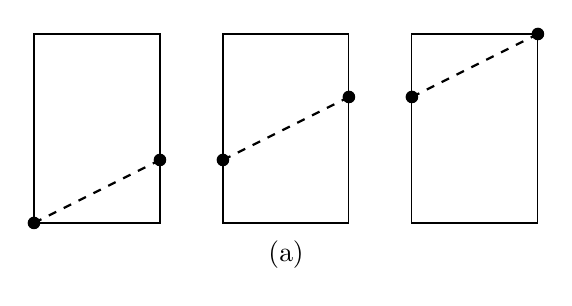
\begin{tikzpicture}[scale=0.8]
  \draw (0,0) rectangle ++(2,3);
  \draw[dashed,thick] (0,0) -- ++(2,1);
  \fill (0,0) circle (0.1);
  \fill (2,1) circle (0.1);

  \draw (3,0) rectangle ++(2,3);
  \draw[dashed,thick] (3,1) -- ++(2,1);
  \fill (3,1) circle (0.1);
  \fill (5,2) circle (0.1);

  \draw (6,0) rectangle ++(2,3);
  \draw[dashed,thick] (6,2) -- ++(2,1);
  \fill (6,2) circle (0.1);
  \fill (8,3) circle (0.1);
  \node at (4, -1/2) {(a)};
\end{tikzpicture}
}

\noindent
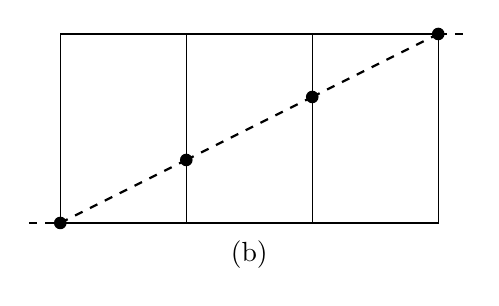
\begin{tikzpicture}[scale=0.8]
  \draw[dashed,thick] (-0.5,0) -- (0,0);
  \fill (0,0) circle (0.1);

  \draw (0,0) rectangle ++(2,3);
  \draw[dashed,thick] (0,0) -- ++(2,1);
  \fill (2,1) circle (0.1);

  \draw (2,0) rectangle ++(2,3);
  \draw[dashed,thick] (2,1) -- ++(2,1);
  \fill (4,2) circle (0.1);

  \draw (4,0) rectangle ++(2,3);
  \draw[dashed,thick] (4,2) -- ++(2,1);
  \fill (6,3) circle (0.1);

  \draw[dashed,thick] (6,3) -- (6.5,3);
  \node at (3, -1/2) {(b)};
\end{tikzpicture}
~
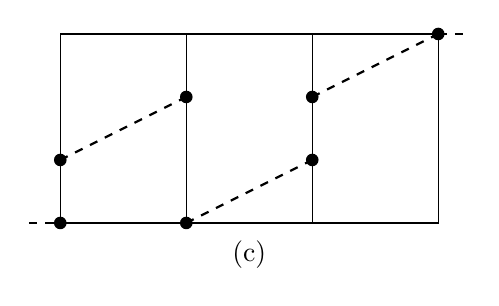
\begin{tikzpicture}[scale=0.8]
  \draw[dashed,thick] (-0.5,0) -- (0,0);
  \fill (0,0) circle (0.1);

  \draw (0,0) rectangle ++(2,3);
  \draw[dashed,thick] (0,1) -- ++(2,1);
  \fill (0,1) circle (0.1);
  \fill (2,2) circle (0.1);

  \draw (2,0) rectangle ++(2,3);
  \draw[dashed,thick] (2,0) -- ++(2,1);
  \fill (2,0) circle (0.1);
  \fill (4,1) circle (0.1);

  \draw (4,0) rectangle ++(2,3);
  \draw[dashed,thick] (4,2) -- ++(2,1);
  \fill (4,2) circle (0.1);
  \fill (6,3) circle (0.1);

  \draw[dashed,thick] (6,3) -- (6.5,3);
  \node at (3, -1/2) {(c)};
\end{tikzpicture}
\caption{
  Part (a) shows a simple schematic for a switch that behaves like $S_3$,
  the symmetric group on three letters.
  The three rectangles can be permuted arbitrarily, but only configuration (b)
  completes the circuit. All other configurations fail to
  complete the circuit (e.g. (c)).
}
\end{figure}

[A schematic for a switch that looks like $D_4$.]


\subsection{Generalizing Spinning}
We can also consider different ways of rearranging the switches.
In a 1995 paper \cite{Ehrenborg1995}, Ehrenborg and Skinner provide a criterion
for which permutations of ordinary, 2-way switches yield a winning strategy.
Rabinovich \cite{Rabinovich2022} settles the problem for switches in a
finite vector space.

For example, one could imagine a ``switch'' that behaves like the symmetric
group $S_3$, consisting of three identical-looking parts that need to be
arranged in a particular order in order for the switch to be on.

Or one could imagine a switch that behaves like the dihedral group of the square,
$D_8$ where the square has a single, unique orientation that completes the circuit.
Or abstractly, one could think of each switch as an abstract group element,
where Player B can multiply by anything they like.

\section{The Wreath Product Model}
\label{sec:WreathModel}
Remind you of the definition of a wreath product, and give examples of how it
models the spinning switches puzzle.
\begin{definition}
  [Literally copied from Rotman]
  Let $D$ and $Q$ be groups,
  let $\Omega$ be a finite $Q$-set, and
  let $K = \prod_{\omega \in \Omega} D_\omega$, where $D_\omega \cong D$
  for all $\omega \in \Omega$.
  Then the \textbf{wreath product} of $D$ by $Q$ denoted by $D \wr Q$,
  is the semidirect product of $K$ by $Q$,
  where $Q$ acts on $K$ by $q \cdot (d_\omega) = d_{q\omega}$ for $q \in Q$ and
  $(d_\omega) \in \prod_{\omega \in \Omega} D_\omega$.
  The normal subgroup $K$ of $D \wr Q$ is called
  the \textbf{base} of the wreath product.
  % Suppose you have two finite groups $G$ and $H$, and a $H$-set $\Omega$,
  % which together form a wreath product $G \wr_\Omega H$ with base \[
  %   K = \prod_{\omega \in \Omega} g_\omega.
  % \]
\end{definition}

TODO: I prefer the Wikipedia version where $q \cdot (d_\omega) = d_{q^{-1}\omega}$

The reason this definition is used is because it models the game well, where
$G$ models the behavior of the switches, $\Omega$ models the switches themselves,
and the way $H$ acts on $\Omega$ models the ways the adversary can ``spin'' the
board.

An element of $(k, h) \in G \wr H$ represents a turn of the game:
Player B chooses $k$ to indicate how they want to modify each of their switches
and then Player A chooses $k$ to indicate how they want to permute the switches.

\begin{example}
  Consider the setup in the original version of the problem consisting of
  two-way switches ($\mathbb Z_2$)
  on the corners of a rotating square
  ($C_4 \cong \langle 0^\circ, 90^\circ, 180^\circ, 270^\circ \rangle$).
  This can be modeled as a game on the wreath product $\mathbb Z_2 \wr C_4$.
  We will use the convention that the base of the wreath product, $K$ is
  ordered upper-left, upper-right, lower-right, lower-left, and the group
  action is specified by degrees in the clockwise direction.

  Consider the following two turns:
  \begin{enumerate}
    \item Turn 1: $((1,0,1,0), 90^\circ) \in \mathbb Z_2 \wr C_4$.
    \begin{enumerate}
      \item Player B toggles the upper-left and lower-right switches.
      \item Player A rotates the table $90^\circ$ clockwise.
    \end{enumerate}
    \item Turn 2: $((1,0,0,0), 180^\circ) \in \mathbb Z_2 \wr C_4$.
    \begin{enumerate}
      \item Player B toggles the upper-left switch.
      \item Player A rotates the table $90^\circ$ clockwise.
    \end{enumerate}
  \end{enumerate}

  As illustrated in Figure \ref{fig:WreathProduct},
  the net result of these two turns is the same as
  a single turn where Player B toggles the upper-left, upper-right, and lower-left
  switches and Player A rotates the board $270^\circ$ clockwise.

  \begin{figure}
    \center
    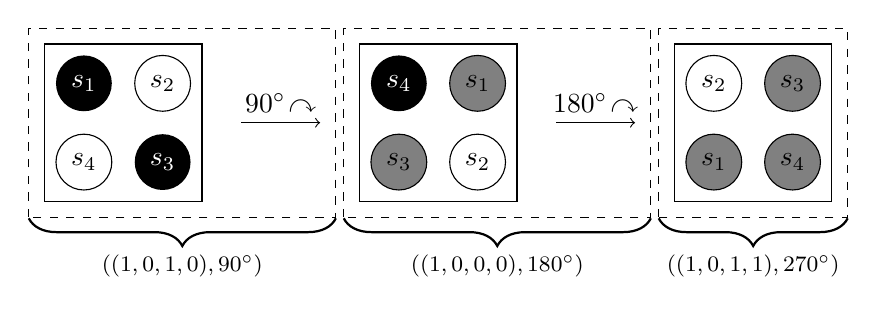
\begin{tikzpicture}
      \draw[dashed] (-0.2,-0.2) rectangle (3.7,2.2);
      \draw [thick,decorate,decoration={brace,amplitude=10pt},yshift=-0.4pt]
        (3.7,-0.2) -- (-0.2,-0.2) node[black,midway,yshift=-0.6cm] {\footnotesize $((1,0,1,0), 90^\circ)$};

      \draw[dashed] (3.8,-0.2) rectangle (7.7,2.2);
      \draw [thick,decorate,decoration={brace,amplitude=10pt},yshift=-0.4pt]
        (7.7,-0.2) -- (3.8,-0.2) node[black,midway,yshift=-0.6cm] {\footnotesize $((1,0,0,0), 180^\circ)$};

      \draw[dashed] (7.8,-0.2) rectangle (10.2,2.2);
      \draw [thick,decorate,decoration={brace,amplitude=10pt},yshift=-0.4pt]
        (10.2,-0.2) -- (7.8,-0.2) node[black,midway,yshift=-0.6cm] {\footnotesize $((1,0,1,1), 270^\circ)$};

      \draw (0,0) rectangle (2,2);
      \node[circle,fill,text=white] at (1/2,3/2) {$s_1$};
      \node[circle,draw] at (3/2,3/2) {$s_2$};
      \node[circle,fill,text=white] at (3/2,1/2) {$s_3$};
      \node[circle,draw] at (1/2,1/2) {$s_4$};
      \draw[->] (2.5,1) -- node[above] {$90^\circ \! \curvearrowright$} (3.5,1) ;

      \draw (4,0) rectangle (6,2);
      \node[circle,fill,text=white] at (9/2,3/2) {$s_4$};
      \node[circle,draw,fill=gray] at (11/2,3/2) {$s_1$};
      \node[circle,draw] at (11/2,1/2) {$s_2$};
      \node[circle,draw,fill=gray] at (9/2,1/2) {$s_3$};

      \draw[->] (6.5,1) -- node[above] {$180^\circ \! \curvearrowright$} (7.5,1) ;

      \draw (8,0) rectangle (10,2);
      \node[circle,draw] at (17/2,3/2) {$s_2$};
      \node[circle,draw,fill=gray] at (19/2,3/2) {$s_3$};
      \node[circle,draw,fill=gray] at (19/2,1/2) {$s_4$};
      \node[circle,draw,fill=gray] at (17/2,1/2) {$s_1$};
    \end{tikzpicture}
    \caption{An illustration of two turns each in the Spinning Switches puzzle,
    modeled as elements of a wreath product.}
    \label{fig:WreathProduct}
  \end{figure}

  The multiplication under the wreath product agrees with this: \[
    ((1,0,1,0), 90^\circ) \cdot ((1,0,0,0), 180^\circ) = ((1,0,1,1), 270^\circ)
  \]
\end{example}

Occasionally it is useful to designate a particular state of the switches as the
on state or the winning state, and ordinarily the identity state is the choice
given for this. However, the existence of a winning strategy does not depend on
a particular choice in the winning state; instead, a winning strategy is
equivalent to a choice of moves that will walk over all of the possible
configuration states, regardless of the choice of the adversaries spin.

\begin{definition}
  A \textbf{switching strategy} is a finite sequence, $\{k_i \in K\}_{i=1}^N$,
  such that for every sequence ${\{h_i \in H\}_{i=1}^N}$,
  \[
    p(\{e_{G \wr H}, (k_1, h_1), (k_1, h_1)\cdot(k_2, h_2), \cdots, (k_1, h_1)\cdot(k_2, h_2)\cdots(k_N, h_N)\}) = K.
  \]
  where $p \colon G \wr_\Omega H \rightarrow K$ is the projection map from the
  wreath product $G \wr_\Omega H$ onto its base $K$.
\end{definition}

% TODO: Variants of this puzzle require more constraints---if you can only change
% $k$ switches,
% or if all of the switches need only to be in the same state,
% or if you can see the states of the switches and player A rotates after you specify what you want.

This definition is useful because it puts the problem into purely algebraic
terms. It is also useful because it abstracts away the initial state of the
switches: regardless of the initial state $k \in K$, a existence of a switching strategy
means that its inverse $k^{-1} \in K$ appears in the sequence.

It's also worth noting that this model can be thought of as a random model or an
adversarial model: the sequence $\{h_i \in H\}$ can be chosen after the sequence
$\{k_i \in K\}$ in a deterministic way randomly.


\begin{enumerate}
  \item Random model to adversarial model
  \item Retroactively changes initial conditions
  \item Spin
  \item Proves lower bound of number of moves
\end{enumerate}

%%%%%%%%%%%%%%%%%%%%%%%%%%%%%%%%%%%%%%%%%%%%%%%%%%%%%%%%%%%%%%%%%%%%%%%%%%%%%%
%
% Historical progress
%
%%%%%%%%%%%%%%%%%%%%%%%%%%%%%%%%%%%%%%%%%%%%%%%%%%%%%%%%%%%%%%%%%%%%%%%%%%%%%%
\section{Historical Progress}
\label{sec:HistoricalProgress}
\subsection{Yehuda (1993) [Roulette wheel]}
\begin{theorem}
  The game on $\mathbb Z_{n} \wr C_{m}$ has a switching strategy if and only if
  $n = p^\alpha$ and $m = p^\beta$ where $p$ is prime and $\alpha$ and $\beta$
  are nonnegative integers. They also deal with words with $q^\beta$ letters
  over $\mathbb F_q$.
\end{theorem}
\subsection{Ehrenborg/Skinner (1995) [Scrambling]}
\begin{theorem}
Interested in fixing $G = \mathbb Z_2$ and looking at permutation
representations of $H$, and determining when switching strategies exist.
They look at a particular ``sub-poset'' of the set partitions of $H$ partially
ordered by refinement, and give a condition which is equivalent to a switching
strategy.
\end{theorem}
\subsection{Sharma/Sidana (2021) [Other related games]}
\subsection{Yuri Rabinovich (2022)}
[Switches are V over $\mathbb F_q$, arbitrary scrambling]

\begin{theorem}
  Let $V$ be a vector space over a finite field $\mathbb F_q$ of characteristic
  $p$, and let $V^+$ be the group under addition.
  Let $G$ be a group that acts linearly and faithfully on $V$.
  Then $G \wr V^+$ has a switching strategy if and only if $G$ is a $p$-group.
\end{theorem}
\section{Reductions}
\label{sec:Reductions}
There are essentially three ways to show that $G \wr H$ does not have a
solution: directly, or via one of two \textit{reductions} (or a combination thereof).

\subsection{Puzzles Without Switching Strategies}
Using results from Rabinovich \cite{Rabinovich2022}, we can give examples of
puzzles that don't have solutions. This section allows us to take those examples
and stretch them into wider families of examples.

\begin{example}
  % Yehuda's ``open game'' makes it clear that $\mathbb Z_2 \wr C_3$ doesn't have a strategy.
  The game $\mathbb Z_2 \wr C_3$ does not have a switching strategy. Here's how to see it...
  \label{ex:NoSolutionZ2C3}
\end{example}

\subsection{Reductions on Switches}
\begin{theorem}
  If $G \wr H$ does not have a switching strategy and $G'$ is a group with
  a quotient $G'/N \cong G$, then ${G'} \wr H$ does not have a switching
  strategy.
  \label{thm:SwitchReduction}
\end{theorem}
\begin{proof}
  I will prove the contrapositive, and suppose that $G' \wr H$ has a
  switching strategy $\{k'_i \in K'\}_{i=1}^N$. The quotient map
  $\varphi\colon G' \mapsto G$
  extends coordinatewise to
  $\hat\varphi \colon K' \mapsto K$.

  The sequence $\{\hat\varphi(k'_i) \in K\}_{i=1}^N$ is a switching strategy on
  $G \wr H$.
  [Say something about how the projection map is ?linear? wrt $\hat\varphi$?
  Say $\phi$ induces a homomorphism from $G' \wr H$?]

  Want to prove \[
    p((\hat\varphi(k'_1),h_1)\dots(\hat\varphi(k'_i),h_i)) =
    \hat\varphi(p'((k'_1,h_1)\dots(k'_i,h_i)))
  \] where $p \colon G \wr H \rightarrow K$ and $p' \colon G' \wr H \rightarrow K'$
\end{proof}
\begin{example}
  We know that $\mathbb Z_2 \wr C_3$ doesn't have a switching strategy.
  This means that $\mathbb Z_6 \wr C_3$ does not have a switching strategy either.
\end{example}
\subsection{Reductions on Spinning}
\begin{theorem}
  If $G \wr H$ does not have a switching strategy and $H'$ is a group with
  a subgroup $A \leq H'$ such that $A \cong H$, then
  $G \wr H'$ does not have a switching strategy.
  \label{thm:SpinReduction}
\end{theorem}
\begin{theorem}
  (Closely related to Theorem \ref{thm:SpinReduction})
  If
  $H'$ is a group with a subgroup $A \leq H'$ such that $A \cong H$,
  $\Omega'$ is an orbit of $\omega \in \Omega$ under $A$, and
  $G \wr_{\Omega'} H$ does not have a switching strategy, then
  $G \wr H'$ does not have a switching strategy.
  \label{thm:SpinReduction2}
\end{theorem}
\begin{proof}
  I will also prove the contrapositive. Assume that $G \wr H'$ does have
  a switching strategy, $\{k_i\}_{i=1}^N$. Then by definition, for any sequence
  $\{h'_i\}_{i=1}^N$, the projection of the sequence \[
    p(\{(k_1, h'_1)\cdot(k_2, h'_2)\cdots(k_i, h'_i)\}_{i=1}^N) = K,
  \] and in particular this is true when $h'_i$ is restricted to be in the
  subgroup $H$. Thus a switching strategy for $G \wr H'$ is also a valid
  switching strategy for $G \wr H$.
\end{proof}
TODO: we have to be careful here, because the simple proof doesn't change the
number of switches, it just makes the set of ``rotations'' smaller.
In the case of the example of $\mathbb Z_2 \wr C_6$, our group action is no
longer transitive, but instead we have two triangular orbits.

TODO: (Something is wrong about this question, but the spirit is right)
Is it true that if $G \wr_\Omega H$ doesn't work then $G \wr_{\Omega'} H'$
doesn't work where $\Omega'$ is any orbit under $N$?
\begin{example}
  We know that $\mathbb Z_2 \wr C_3$ doesn't have a switching strategy.
  This means that $\mathbb Z_2 \wr C_6$ does not have a switching strategy either.
  \begin{figure}
    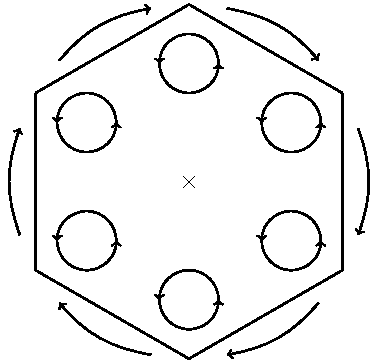
\includegraphics{assets/tikz_Z2C6.pdf}
    \caption{If there were a solution to $\mathbb Z_2 \wr C_6$, then there
    would be a solution to ...}
  \end{figure}
\end{example}

%%%%%%%%%%%%%%%%%%%%%%%%%%%%%%%%%%%%%%%%%%%%%%%%%%%%%%%%%%%%%%%%%%%%%%%%%%%%%%
%
% Switching strategies on p-groups
%
%%%%%%%%%%%%%%%%%%%%%%%%%%%%%%%%%%%%%%%%%%%%%%%%%%%%%%%%%%%%%%%%%%%%%%%%%%%%%%
\section{Switching Strategies on \texorpdfstring{$p$}{p}-Groups}
\label{sec:pGroupStrategy}
\begin{theorem}
  The wreath product $G \wr H$ has a switching strategy if there exists a
  normal subgroup $N \trianglelefteq G$ such that both $N \wr H$ and
  $G/N \wr H$ have switching strategies.
\end{theorem}
\begin{proof}
  Let $S_{G/N} = \{k_i^{G/N} \in K_{G/N}\}$ denote the switching strategy for $G/N \wr H$, and
  let $S_{N} = \{k_i^N \in K_{N}\}$ denote the switching strategy for $N \wr H$.

  First, we partition $G$ into $|G|/|N| = m$ cosets of $N$: \[
    G = g_1N \sqcup g_2N \sqcup \dots \sqcup g_mN.
  \]

  From the switching strategy $\{k_i^{G/N} \in K_{G/N}\}$,
  we can get a sequence $S_{G'} = \{k_i' \in K_G\}$
  by picking the coset representatives coordinatewise.

  This sequence is not itself a switching strategy, but it does ``hit'' all
  combinations of cosets. That is, for every ``spinning sequence'' $\{h_i \in H\}$,
  and sequence of cosets $(g_{i_1}H, g_{i_2}H, \dots, g_{i_m}H)$, there exists
  an index $n$ such that \[
    p((k_1', h_1) \dots (k_n', h_n)) \in g_{i_1}H \times g_{i_2}H \times \dots \times g_{i_m}H
  \]

  Now if we intersperse $S_G' \circledast S_N$, this forms a
  switching strategy because ... \[
    S_G' \circledast S_N = (\underbrace{k^N_1, k^N_2, \dots, k^N_{n_N}}_{B_0}, \underbrace{k'_1, k^N_1, k^N_2, \dots, k^N_{n_N}}_{B_1}, \dots, \underbrace{k'_{n'}, k^N_1, k^N_2, \dots, k^N_{n_N}}_{B_{n'}})
  \]

  The partial products that end in block $B_i$ all have switches in the same
  cosets of $N$, and the $S_N$ strategy then hits all elements of $K_G$ that
  belong to that combination of cosets.

  % First, we choose representatives ${g_1, g_2, \dots, g_{m}}
\end{proof}
\begin{theorem} \cite{Rabinovich2022}
  Assume that a finite group $H$ acts linearly and faithfully on a vector space
  $V$ over a finite field $\mathbb F_q$ of characteristic $p$.
  Then $(G, V)$ is friendly if and only if $G$ is a $p-group$.
\end{theorem}
\begin{corollary}
  If $H$ is a finite group that acts faithfully on $\Omega$, then the wreath product
  $G \wr H$ has a switching strategy whenever $|G| = p^n$ for some $n$.
\end{corollary}
\begin{proof}
  If $|G| = p^n$, then either $G \cong \mathbb{Z}_p$ or $G$ is not simple.
  If $G \cong \mathbb{Z}_p$, then there exists a strategy. Otherwise,
  $G$ is not simple, so choose a normal subgroup $N$ of order $|N| = p^t$
  which gives a quotient $G/N$ with order $|G/N| = p^{n-t}$. Then the
  result follows by induction.
\end{proof}
\begin{corollary}
  Based on the above construction, if $|G| = p^n$, then $G \wr C_{p^\ell}$
  has a palindromic strategy of length $p^{n p^\ell}-1$.
\end{corollary}
\begin{proof}
  Is this true for general $H \neq C_{p^\ell}$?
\end{proof}

%%%%%%%%%%%%%%%%%%%%%%%%%%%%%%%%%%%%%%%%%%%%%%%%%%%%%%%%%%%%%%%%%%%%%%%%%%%%%%
%
% Switching strategies on permutations
%
%%%%%%%%%%%%%%%%%%%%%%%%%%%%%%%%%%%%%%%%%%%%%%%%%%%%%%%%%%%%%%%%%%%%%%%%%%%%%%
\section{Switching Strategies on Other Wreath Products}
\label{sec:OtherSwitchingStrategies}

So far, the literature has only contained examples of spinning strategies on
wreath products that are themselves $p$-groups:
$|G \wr_\Omega H| = |G|^{|\Omega|} \cdot |H|$, where $H$ acts faithfully.

Of course, if $H = \textbf{1}$ is the trivial group, then
$G \wr \mathbf{1} \cong G$ has a switching strategy even if $G$ is not a $p$-group.
(In fact, it has $(|G|-1)!$ switching strategies!)

\subsection{\texorpdfstring{$S_3 \wr C_2$}{Two copies of the symmetric group on three letters}}
Here's an example.
\begin{example}
  If $a \in S_3$, let $a_1$ mean multiplying one of the two copies by $a$ and
  $a_2$ mean multiplying both of the copies by $a$. Then the following is
  a strategy:
  \begin{align*}
    (12)_2(13)_2(12)_2(13)_2(12)_2 \\
    &(12)_1 \\
    (12)_2(13)_2(12)_2(13)_2(12)_2 \\
    &(13)_1 \\
    (12)_2(13)_2(12)_2(13)_2(12)_2 \\
    &(12)_1 \\
    (12)_2(13)_2(12)_2(13)_2(12)_2 \\
    &(13)_1 \\
    (12)_2(13)_2(12)_2(13)_2(12)_2 \\
    &(12)_1 \\
    (12)_2(13)_2(12)_2(13)_2(12)_2
  \end{align*}
  \label{ex:TwoSymmetricGroups}
\end{example}
In general, if you can walk through $G$ with elements of order $2$, then
there is a strategy.
%%%%%%%%%%%%%%%%%%%%%%%%%%%%%%%%%%%%%%%%%%%%%%%%%%%%%%%%%%%%%%%%%%%%%%%%%%%%%%
%
% Open questions
%
%%%%%%%%%%%%%%%%%%%%%%%%%%%%%%%%%%%%%%%%%%%%%%%%%%%%%%%%%%%%%%%%%%%%%%%%%%%%%%
\section{Open questions}
\label{sec:OpenQuestions}
\subsection{Palindromic switching strategies}
In all known examples, when there exists a switching strategy $S$,
there exists a \textit{palindromic} switching strategy
$S' = \{k'_i \in K\}_{i=0}^N$
such that $k'_i = k'_{N-i}$ for all $i$.
\begin{conjecture}
  Whenever $G \wr H$ has a switching strategy, it also has a palindromic switching
  strategy.
\end{conjecture}

I'm interested in the answer even in the case of $G \wr \mathrm{1} \equiv G$.

(\href{https://math.stackexchange.com/q/3706654/121988}{MSE})

\subsection{Quasigroup switches}
In the paper we modeled switches as groups.
This is because groups have desirable properties: \begin{enumerate}
  \item Closure. Regardless of which state a switch is in, modifying the state is the set of states.
  \item Identity. We don't have to toggle a switch on a given turn.
  \item Inverses. If a switch is off, we can always turn it on.
\end{enumerate}

It turns out that we don't need the axiom of associativity,
because the sequencing is naturally what computer scientists call
``left associative''. Thus, we can model switches a bit more generally as
\textit{loops} (i.e. quasigroups with identity.)

\subsection{Expected number of turns}
If we're to play the game uniformly at random, we're equally likely to win on
any turn (of course, we never choose the ``do nothing'' move), so the expected
number of moves is $|K| - 1$.

If there's a switching strategy, we're equally likely to win on any turn, so
the expected number is $(N+1)/2$ with an $N$ move strategy. In all cases,
when a strategy is known, a \textit{minimal} strategy is known, so this is
reduced to $|K|/2$.

\begin{conjecture}
  Whenever $G \wr H$ has a switching strategy, it also has a minimal switching
  strategy.
\end{conjecture}

For setups that don't have a switching strategy, what is an (infinite) strategy
that minimizes the expected number of turns?
We can always do a bit better than the naive play by saying never do
$(g,g, ..., g) \in K$ followed by $(g^{-1},g^{-1}, ..., g^{-1}) \in K$.

\begin{quote}
  This puzzle reached me via Sasha Barg of the University of Mary-
  land, but seems to be known in many places. Although no fixed number of steps
  can guarantee turning the bulb on in the three-switch version, a smart randomized
  algorithm can get the bulb on in at most $5 \frac{5}{7}$ steps on average, against any strategy
  by an adversary who sets the initial configuration and turns the platform. \cite{Winkler2021}
\end{quote}

\subsection{Multiple moves between each turn}
We could modify the puzzle so that the adversary's spinning sequence
$\{h_i \in H\}$ is constained so that $h_i = e_H$ whenever $i \ncong 0 \bmod k$;
that is, the adversary can only spin every $k$ turns. For any finite setup
$G \wr H$, there exists $k$ such that Player B can win.
(For example, take $k > |K|$ so that Player B can just do a walk of $K$.)

How can you compute the minimum $k$ such that Player B has a strategy for each
choice of $G \wr H$? This is an interesting statistic.

\subsection{Different sorts of buttons}
We could imagine a square board with different sorts of buttons---for instance
one of the corners has an ordinary 2-way button and another has a 3-way button
and so on. When do such setups have a switching strategy.
(We can also put this problem into purely algebraic terms.)
Of course, if one is a button and another is like $S_3$ then it's not clear how
to keep them indistinguishable to Player B. In the case of the buttons,
we can have $\mathbb Z$ act on either of them.

\subsection{Counting switching strategies}
Is there a good way to count the number of switching strategies?
How about up to the action of $H$?

In the case of $S_3 \wr \bf{1}$, I counted the palindromic switching
strategies, which can give a lower bound on the number of palindromic
switching strategies of $S_3 \wr C_2$.
(\href{https://math.stackexchange.com/q/3717562/121988}{MSE})

\subsection{Yehuda's ``open game''}
Yehuda has an ``open game'' version of the puzzle that goes like this:
Everyone can see the state of the board.
Player B says what moves (positionally) they want to make.
Player A rotates the board however they see fit \textit{then} applies Player
B's move.
\begin{conjecture}
  Player B can always win by repeatedly choosing the inverse of the board.
\end{conjecture}

\begin{example} This strategy works for $\mathbb Z_2 \wr C_4$. Here's one example.
  \begin{itemize}
    \item The initial state of the board is one switch off and all of the others on.
    \item Player B says to turn on the off switch.
    \item Player A turns the board in order to turn off an adjacent switch.
    \item Player B says to turn on those two adjacent switches.
    \item Player A turns the board in order to toggle one of the switches, leaving one diagonal on and one off.
    \item Player B says to turn on those two diagonal swtiches.
    \item Player A rotates the board to instead turn off the two on switches so that all switches are off.
    \item Player B says to turn on all of the switches.
    \item Player A knows that rotating the board does not do anything, so they turn on all of the switches.
    \item Player B wins.
  \end{itemize}
\end{example}

This strategy also works for $\mathbb Z_3 \wr C_3$.

\subsection{Generalizations of \texorpdfstring{$S_3 \wr C_2$}{Two interchangeable copies of the symmetric group}}

In Example \ref{ex:TwoSymmetricGroups}, we constructed a strategy for $S_n \wr C_2$,
by exploiting the fact that $S_n$ can be generated by elements of order $2$.

\begin{conjecture}
  There exists a switching strategy for $S_n \wr C_4$.
\end{conjecture}

\begin{conjecture}
  There exists a switching strategy for $A_n \wr C_3$.
\end{conjecture}

The generalization of this conjecture, which is as likely to be false as it is
to be true doesn't have evidence to support it.
\begin{conjecture}
  If $G$ can be generated by elements of order $p^n$, and $H$ is a $p$-group
  acting faithfully on the set of switches $\Omega$, then $G \wr_\Omega H$ has
  a switching strategy.
\end{conjecture}

\chapter{Permutation Statistics}
\label{cha:PermutationStatistics}

In this paper, we study permutations $\pi \in S_n$ with exactly $m$ transpositions.
In particular, we are interested in the expected value of $\pi(1)$ when such
permutations are chosen uniformly at random. When $n$ is even, this expected value
is approximated closely by $(n+1)/2$, with an error term that is related to the number isometries
of the $(n/2-m)$-dimensional hypercube that move every face.
Furthermore, when $k \mid n$, this construction generalizes to allow us to compute
the expected value of $\pi(1)$ for permutations
with exactly $m$ $k$-cycles. In this case, the expected value has an
error term which is related instead to the number derangements of the
generalized symmetric group $S(k,n/k-m)$.

When $k$ does not divide $n$, the expected value of $\pi(1)$ is precisely
$(n+1)/2$.
Indirectly, this suggests the existence of a reversible algorithm
to insert a letter into a permutation which preserves the number of $k$-cycles,
which we construct.

\section{Background}
\label{section:background}

In 2010, Mark Conger \cite{conger} proved that a permutation
with $k$ descents has an expected first letter of $\pi(1) = k + 1$,
independent of $n$.
This paper has the same premise, but with a different permutation statistic:
the number of $k$-cycles of a permutation.

This section, (Section \ref{section:background}) provides an overview of where
we're headed, and includes an critical example that will hopefully spark the
reader's curiosity and motivate the remainder of the paper.

Section \ref{section:recursiveStructure} establishes some recurrence relations for
the number of permutations in $S_n$ with a given number of $k$-cycles.
It also contains a theorem that gives an explicit way to compute the expected
value of the first letter based on these counts.

Section \ref{section:wreathProduct} describes an explicit correspondence
between $k$-cycles of permutations in $S_{kn}$ and fixed points of elements of the generalized
symmetric group $(\mathbb{Z}/k\mathbb{Z}) \wr S_n$. Using generating functions and results
from the previous section, this shows that the expected value of $\pi(1)$ of a
permutation with a given number of $k$-cycles is intimately connected to the
number of derangements of a generalized symmetric group.

While Section \ref{section:wreathProduct} emphasizes the case of $S_{kn}$,
Section \ref{section:bijection} looks at $S_N$ where $k \nmid N$. Here, the
expected value of $\pi(1)$ is simply $(N+1)/2$, which agrees with the expected
value of the first letter of a uniformly chosen $N$-letter permutation with
no additional restrictions. This fact together with the main
theorem from Section \ref{section:recursiveStructure} implies the existence of a
bijection $\varphi_k \colon S_{N-1} \times [N] \rightarrow S_N$ that preserves the
number of $k$-cycles whenever $k \nmid N$. Section \ref{section:bijection}
constructs such a bijection explicitly, and proves that it has the desired
properties.

\subsection{Motivating Examples}

In support of the first examples, we start by defining the first bit of notation.
\begin{definition}
  Let $C_k(n,m)$ denote the number of permutations $\pi \in S_n$ such that
  $\pi$ has exactly $m$ $k$-cycles.
\end{definition}

These theorems---and many of the following lemmas---were discovered by looking
at examples such as the following, written in both one-line and cycle notation:

\begin{example}
\label{ex:fourLettersTwoCycles}
  There are $C_2(4,0) = 15$ permutations in $S_4$ with no $2$-cycles:
  \begin{alignat*}{5}
    1234 &= (1)(2)(3)(4) \hspace{0.5 cm}
    && 2314 = (312)(4)\hspace{0.5 cm}
    && 3124 = (321)(4)\hspace{0.5 cm}
    && 4123 = (4321) \\
%
    1342 &= (1)(423) \hspace{0.5 cm}
    && 2341 = (4123) \hspace{0.5 cm}
    && 3142 = (4213) \hspace{0.5 cm}
    && 4132 = (421)(3)\\
%
    1423 &= (1)(432) \hspace{0.5 cm}
    && 2413 = (4312) \hspace{0.5 cm}
    && 3241 = (2)(413) \hspace{0.5 cm}
    && 4213 = (2)(431) \\
%
    & \
    && 2431 = (3)(412)  \hspace{0.5 cm}
    && 3421 = (4132) \hspace{0.5 cm}
    && 4312 = (4231)
  \end{alignat*}
  There are $C_2(4,1) = 6$ permutations in $S_4$ with exactly one $2$-cycle:
  \begin{alignat*}{3}
    1243 &= (1)(2)(43) \hspace{1cm}
    && 2134 = (21)(3)(4) \\
%
    1324 &= (1)(32)(4) \hspace{1cm}
    && 3214 = (2)(31)(4)\\
%
    1432 &= (1)(3)(42) \hspace{1cm}
    && 4231 = (2)(3)(41)
  \end{alignat*}
  And there are $C_2(4,2) = 3$ permutations in $S_4$ with exactly two $2$-cycles,
  \begin{equation*}
    2143 = (21)(43) \hspace{1cm}
    3412 = (31)(42) \hspace{1cm}
    4321 = (32)(41).
  \end{equation*}
  By averaging the first letter over these examples, we can
  compute that \begin{alignat*}{3}
    &\mathbb{E}[\pi(1)\, |\, \pi \in S_4 \text{ has no } 2 \text{-cycles}\,]
      &&= \frac{3(1) + 4(2 + 3 + 4)}{15}
      &&= \frac{13}{5},
    \\
    &\mathbb{E}[\pi(1)\, |\, \pi \in S_4 \text{ has exactly } 1\ 2 \text{-cycle}]
      &&= \frac{3(1) + (2 + 3 + 4)}{6}
      &&= 2, \text{ and}
    \\
    &\mathbb{E}[\pi(1)\, |\, \pi \in S_4 \text{ has exactly } 2\ 2 \text{-cycles}\,]
      &&= \frac{2 + 3 + 4}{3}
      &&= 3.
  \end{alignat*}
\end{example}
The table in Figure \ref{fig:twoCyclesTable} gives the expected value of $\pi(1)$ given that
$\pi \in S_n$ and has exactly $m$ $2$-cycles in its cycle decomposition.
Notice that when $i$ is odd, row $i$ has a constant value of $(i+1)/2$. Also
notice that the number in position $(i,j)$ has the same denominator as the
number in position $(i+2, j+1)$, and that these denominators increase with $n$.
The sequence of denominators begins \begin{equation}
  1, 5, 29, 233, 2329, 27949, \dots,
\end{equation}
which agrees with the type B derangement numbers,
sequence A000354 in the On-Line Encyclopedia of Integer Sequences (OEIS) \cite{oeis}.
In other words, the denominators in the table appear to be related to
the symmetries of the hypercube that move every facet.
\begin{table}
  \[
  \begin{array}{|ll|l|l|l|l|l|l|l|l|l|l|}
  \hline
  & & \multicolumn{7}{|c|}{m} \\ \cline{3-9}
  & & 0 & 1 & 2 & 3 & 4 & 5 & 6 \\ \hline
  \multirow{8}{*}{$n$}
  & \n{1}  & 1/1          &            &          &        &      &     &     \\ \cline{2-4}
  & \n{2}  & 1/1          & 2/1        &          &        &      &     &     \\ \cline{2-4}
  & \n{3}  & 2/1          & 2/1        &          &        &      &     &     \\ \cline{2-5}
  & \n{4}  & 13/5         & 2/1        & 3/1      &        &      &     &     \\ \cline{2-5}
  & \n{5}  & 3/1          & 3/1        & 3/1      &        &      &     &     \\ \cline{2-6}
  & \n{6}  & 101/29       & 18/5       & 3/1      & 4/1    &      &     &     \\ \cline{2-6}
  & \n{7}  & 4/1          & 4/1        & 4/1      & 4/1    &      &     &     \\ \cline{2-7}
  & \n{8}  & 1049/233     & 130/29     & 23/5     & 4/1    & 5/1  &     &     \\ \cline{2-7}
  & \n{9}  & 5/1          & 5/1        & 5/1      & 5/1    & 5/1  &     &     \\ \cline{2-8}
  & \n{10} & 12809/2329   & 1282/233   & 159/29   & 28/5   & 5/1  & 6/1 &     \\ \cline{2-8}
  & \n{11} & 6/1          & 6/1        & 6/1      & 6/1    & 6/1  & 6/1 &     \\ \cline{2-9}
  & \n{12} & 181669/27949 & 15138/2329 & 1515/233 & 188/29 & 33/5 & 6/1 & 7/1 \\ \cline{2-9}
  & \n{13} & 7/1          & 7/1        & 7/1      & 7/1    & 7/1  & 7/1 & 7/1 \\ \hline
  \end{array}
  \]
  \caption[The expected value of $\pi(1)$ for $\pi \in S_n$ with $m$ $2$-cycles.]{
    A table of the expected value of the first letter of $\pi \in S_n$ with
    exactly $m$ $2$-cycles,
    ${\mathbb{E}[\pi(1)\, |\, \pi \in S_n \text{ has exactly } m\ 2 \text{-cycles}\,]}$.
  }
  \label{fig:twoCyclesTable}
\end{table}
\section{Structure of permutations with \texorpdfstring{$m$}{m} \texorpdfstring{$k$}{k}-cycles}
\label{section:recursiveStructure}
This section is about connecting the number of permutations with a given number of
$k$-cycles to the expected value of the first letter. Saying this, it is
appropriate to start with a 1944 theorem of Goncharov that, by the principle of
inclusion/exclusion, gives an explicit formula that counts the number of such
permutations.
\subsection{Counting permutations based on cycles}
\begin{theorem}[\cite{goncharov}, \cite{arratia}]
  \label{GoncharovTheorem}
  The number of permutations in $S_n$ with exactly $m$ $k$-cycles is given by
  the following sum, via the principle inclusion/exclusion:
  \begin{equation}
    C_k(n,m)
    = \frac{n!}{m!k^m}\sum_{i=0}^{\lfloor n/k \rfloor - m} \frac{(-1)^i}{i!\,k^i}.
  \end{equation}
  \label{eq:Goncharov}
\end{theorem}

\begin{corollary}
  For $k \nmid n$, there are exactly $n$ times as many permutations in $S_n$
  with exactly $m$ $k$-cycles than there are in $S_{n-1}$.
  When $k \mid n$, there is an explicit formula for the difference.
  \label{cor:bijectionDifference}
  \begin{numcases}{C_k(n, m) - nC_k(n-1,m) = }
    0 & $k \nmid n$ \label{eq:bijectionDifference0}
    \\
    \displaystyle\frac{n!(-1)^{\frac nk - m}}{(n/k)! \, k^{\frac nk}}\binom{n/k}{m} & $k \mid n$
    \label{eq:bijectionDifference1}
  \end{numcases}
  \label{eq:bijectionDifference}
\end{corollary}
\begin{proof}
  When $k \nmid n$,
  $\displaystyle \left\lfloor \frac{n}{k}\right\rfloor = \left\lfloor \frac{n-1}{k}\right\rfloor$,
  so the bounds on the sums are identical and the result follows directly \begin{align}
    \frac{n!}{m!k^m}\sum_{i=0}^{\lfloor n/k \rfloor - m} \frac{(-1)^i}{i!\,k^i}
    - n\left(\frac{(n-1)!}{m!k^m}\sum_{i=0}^{\lfloor (n-1)/k \rfloor - m} \frac{(-1)^i}{i!\,k^i}\right)
    = 0.
  \end{align}
  Otherwise, when $k \mid n$,
  $\displaystyle \left\lfloor \frac{n-1}{k}\right\rfloor = \frac{n}{k} - 1$, so
  \begin{align}
    \nonumber
    &\frac{n!}{m!k^m}\sum_{i=0}^{n/k - m} \frac{(-1)^i}{i!\,k^i}
    - n\left(\frac{(n-1)!}{m!k^m}\sum_{i=0}^{n/k - 1 - m} \frac{(-1)^i}{i!\,k^i}\right) \\[10pt]
    \nonumber
    &\hspace{4cm}= \frac{n!}{m!k^m}\left(\frac{(-1)^{n/k - m}}{(n/k - m)!k^{n/k - m}}\right) \\[10pt]
    \nonumber
    &\hspace{4cm}= \frac{n!(-1)^{n/k - m}}{(n/k - m)!m!k^{n/k}} \\[10pt]
    &\hspace{4cm}= \frac{n!(-1)^{\frac nk - m}}{(n/k)! \, k^{n/k}}\binom{n/k}{m}.
  \end{align}
\end{proof}
See Section \ref{section:bijection} for a bijective proof of Equation
\ref{eq:bijectionDifference0}.

\subsection{Permutations by first letter}
In order to compute the expected value of the first letter of a permutation,
it is useful to be able to compute the number of permutations that have a given
number of $k$-cycles \textit{and} a given first letter.
\begin{definition}
  Let $C_k^{(a)}(n,m)$ be the number of permutations $\pi \in S_n$ that
  have exactly $m$ $k$-cycles and $\pi(1) = a$.
\end{definition}
The expected value of $\pi(1)$ with a given number of
$k$-cycles
% can be computed in exactly the same manner as in Example
% \ref{ex:fourLettersTwoCycles}.
% \begin{definition}
%   \label{weightedAverage}
%   The expected value of $\pi(1)$ given $\pi \in S_n$ with $m$ $k$-cycles
is
  \begin{equation}
    \mathbb{E}[\pi(1)\, |\, \pi \in S_n \text{ has exactly } m\ k \text{-cycles}\,] =
    \frac{1}{C_k(n, m)}\sum_{a=1}^n a C_k^{(a)}(n, m).
    \label{eq:weightedAverage}
  \end{equation}
The following three lemmas compute $C_k^{(a)}(n,m)$ from $C_k(n,m)$.
\begin{proposition}
  \label{cyc1Recurrence}
  For all $k > 1$, the number of permutations in $S_n$ starting with $1$ and
  having $m$ $k$-cycles is equal to the number of permutations in $S_{n-1}$ with
  $m$ $k$-cycles: \begin{equation}
    C_k^{(1)}(n,m) = C_k(n-1, m).
  \end{equation}
\end{proposition}
\begin{proof}
  The straightforward bijection from $\{\pi \in S_n : \pi(1) = 1\}$ to $S_{n-1}$
  given by deleting $1$ and relabeling preserves the number of $k$-cycles for
  $k > 1$.
\end{proof}
\begin{proposition}
  \label{allSame}
  For all $a, b \geq 2$, the number of permutations having $k$-cycles
  and starting with $a$ are the same as the number of those starting with $b$:
  \begin{equation}
    C_k^{(2)}(n,m) = \cdots = C_k^{(a)}(n,m) = \cdots = C_k^{(b)}(n,m) = \cdots = C_k^{(n)}(n,m).
  \end{equation}
\end{proposition}
\begin{proof}
  Since the permutations under consideration do not fix $1$,
  conjugation by $(ab)$ is an isomorphism which takes all words starting
  with $a$ to words starting with $b$ without changing the cycle structure.
\end{proof}
\begin{lemma}
  \label{cycRecurrenceWithFixedBeginning}
  For all $2 \leq a \leq n$, \begin{align}
    C_k^{(a)}(n,m) = \frac{C_k(n, m) - C_k(n-1, m)}{n - 1}.
  \end{align}
\end{lemma}
\begin{proof}
  Since \begin{equation}
    C_k(n, m) = C_k^{(1)}(n, m) + C_k^{(2)}(n, m) + \dots + C_k^{(n)}(n, m),
  \end{equation} using Proposition \ref{allSame}, for the last $(n-1)$ terms,
  this can be rewritten as \begin{equation}
    C_k(n, m) = C_k^{(1)}(n, m) + (n-1)C_k^{(a)}(n, m).
  \end{equation}
  Solving for $C_k^{(a)}(n, m)$ and using the substitution from Proposition
  \ref{cyc1Recurrence} gives the desired result.
\end{proof}
Now, equipped with explicit formulas for $C_k^{(a)}(n,m)$ and $C_k(n,m)$, we
can compute the expected value of $\pi(1)$ for $\pi \in S_n$ with exactly $m$
$k$-cycles.
\subsection{Expected value of first letter}
\begin{theorem}
  \label{firstTheorem}
  For $k > 1$, the expected value of the first letter of a permutation
  $\pi \in S_n$ with $m$ $k$-cycles is given by \begin{align}
    &\mathbb E[\pi(1)\ \mid\ \pi \in S_n \text{ has exactly } m\ k\text{-cycles}\,]
    \nonumber
    \\
    & \hspace{4cm} = \frac n2\left(1 - \frac{C_k(n-1,m)}{C_k(n,m)}\right) + 1.
  \end{align}
\end{theorem}
\begin{proof}
  % Recall Equation \ref{eq:weightedAverage}, \begin{equation}
  %   \mathbb E[\pi(1)\ \mid\ \pi \in S_n \text{ has exactly } m\ k\text{-cycles}\,] =
  %   \frac{1}{C_k(n, m)}\sum_{a = 1}^n aC_k^{(a)}(n, m).
  % \end{equation}
  Using Proposition \ref{allSame}, we can consolidate all but the first term of
  the sum in Equation \ref{eq:weightedAverage} \begin{align}
    &\sum_{a = 1}^n aC_k^{(a)}(n, m) \\
    &\hspace{1cm}= C_k^{(1)}(n,m) + \sum_{a = 2}^n aC_k^{(n)}(n, m) \\
    % &\hspace{1cm}= C_k^{(1)}(n,m) + C_k^{(n)}(n, m)\sum_{a = 2}^n a \\
    &\hspace{1cm}= C_k^{(1)}(n,m) + \frac{(n-1)(n+2)}{2} C_k^{(n)}(n, m) \\
  % \end{align}
  % Now using the formulas in Proposition \ref{cyc1Recurrence} and Lemma
  % \ref{cycRecurrenceWithFixedBeginning} \begin{align}
    % &\sum_{a = 1}^n aC_k^{(a)}(n, m)
    % \nonumber
    % \\
    &\hspace{1cm}=
    C_k(n-1,m) + \frac{(n-1)(n+2)}{2}\left(
      \frac{C_k(n, m) - C_k(n-1, m)}{n - 1}
    \right) \\
    &\hspace{1cm}= \left(\frac{n}{2} + 1\right) C_k(n,m) - \frac n2C_k(n-1,m).
  \end{align}
  Dividing by $C_k(n,m)$ yields the result.
\end{proof}
\begin{corollary}
  \label{cor:kNotDivideN}
  When $k \nmid n$, $C_k(n,m) = nC_k(n-1,m)$ by Equation \ref{eq:bijectionDifference0},
  so \begin{equation}
    \mathbb E[\pi(1)\ \mid\ \pi \in S_n \text{ has exactly } m\ k\text{-cycles}\,] = \frac{n}{2}\left(1 - \frac{1}{n}\right) + 1 = \frac{n+1}{2}.
  \end{equation}
\end{corollary}
Together with Theorem \ref{GoncharovTheorem}, this theorem and its corollary
provides our first formula for the expected value of $\pi(1)$ that
performs exponentially better than brute force.

\subsection{Identities for counting permutations with given cycle conditions}
Both in practical terms (if computing the expected value of $\pi(1)$ by hand or
optimizing an algorithm) and in a theoretical sense, the following recurrence is
simple and useful.

\begin{lemma}
  \label{cycleRecursion}
  For $n < mk$ or $m < 0$, $C_k(n, m) = 0$. Otherwise,
  for all $k, m \geq 1$ \begin{equation}
    mC_k(n, m) = (k-1)!\binom{n}{k}C_k(n-k, m-1).
  \end{equation}
\end{lemma}
While this can be proven directly by the algebraic manipulation of the
identity in Theorem \ref{GoncharovTheorem}, a bijective proof has been
included here because it is natural and may be of interest.
\begin{proof}
  Let \begin{equation}
  \mathcal C_k(n, m) = \{ \pi \in S_n\,\mid\,\pi \text{ has exactly } m\ k \text{-cycles}\}.
  \end{equation}
  Then consider the two sets, whose cardinalities match the left- and
  right-hand sides of the equation above:
  \begin{align}
    X^{L}_{n,m,k} &= \{ (\pi, c) \mid \pi \in \mathcal C_k(n, m), c \text{ a distinguished } k\text{-cycle of } \pi \}. \\
    X^{R}_{n,m,k} &= \{ (\sigma, d) \mid \pi \in \mathcal C_k(n-k, m-1), d \text{ an } n\text{-ary necklace of length } k\}.
  \end{align}
  The first set, $X^{L}_{n,m,k}$, is constructed by taking a permutation in
  $\mathcal C_k(n,m)$ and choosing one of its $m$ $k$-cycles to be distinguished, so
  $\#X^{L}_{n,m,k} = mC_k(n,m)$.

  In the second set, $X^{R}_{n,m,k}$, the two parts of the tuple are independent.
  There are $C_k(n-k, m-1)$ choices for the permutation $\sigma$ and $(k-1)!\binom{n}{k}$
  choices for the necklace $d$.
  Thus $\#X^{R}_{n,m,k} = (k-1)!\binom{n}{k}C_k(n-k, m-1)$.

  Now, consider the map $\varphi \colon X^{L}_{n,m,k} \rightarrow X^{R}_{n,m,k}$
  which removes the distinguished $k$-cycle and relabels the remaining $n - k$
  letters as $\{1, 2, \dots, n - k\}$, preserving the relative order:
  \begin{equation}
    (\pi_1\pi_2 \cdots \pi_\ell, \pi_i) \xmapsto{\varphi} (\pi'_1\pi'_2 \cdots \pi'_{i-1}\pi'_{i+1} \cdots \pi'_\ell, \pi_i)
  \end{equation} where $\pi'_i$ is $\pi_i$ after relabeling.

  By construction, $\sigma$ has one fewer $k$-cycle and $k$ fewer letters
  than $\pi$.

  The inverse map is similar. To recover $\pi$, increment the letters of $\sigma$ appropriately
  and add the necklace $d$ back in as the distinguished cycle.
  Thus $\varphi$ is a bijection and $\#X^{L}_{n,m,k} = \#X^{R}_{n,m,k}$.
\end{proof}
\begin{example}
  Suppose $\pi = (423)\mathbf{(61)}(75)$ in cycle notation with $(61)$ distinguished.
  Then \begin{align}
    \varphi((423)(61)(75), (61)) = ((312)(54), (61))
  \end{align} under the bijection $\varphi$, described in the proof of
  Lemma \ref{cycleRecursion}.
\end{example}
% As the above lemma suggests, we find particular interest in the case
% where $k \mid n$. Also, we can understand much of the structure of $C_k(n,m)$ by
% understanding the structure of $C_k(n', 0)$.
% This is closely related to the generating function in Theorem \ref{derangementEGF}
The recurrence in Lemma \ref{cycleRecursion} suggests that understanding
$C_k(n,m)$ is related to understanding $C_k(n-km, 0)$,
the permutations of $S_{n-km}$ with no $k$-cycles.
On the other hand,
Corollary \ref{cor:bijectionDifference} suggests that the case where $k \mid n$
has some of the most intricate structure.
We can, of course, combine these two observations and analyze the case of
$C_k(kn, 0)$, which has a particularly simple generating function, which will
show up again in a different guise.
\begin{lemma}
  For $k \geq 2$,
  \label{cycleEGF}
  \begin{equation}
    \sum_{n=0}^\infty \frac{C_k(kn, 0)k^n}{(kn)!}x^n
    = \frac{\exp(-x)}{1-kx}.
  \end{equation}
\end{lemma}
\begin{proof}
  By substitution of $C_k(kn, 0)$ via the identity in Theorem \ref{GoncharovTheorem},
  \begin{align}
    \sum_{n=0}^\infty \frac{C_k(kn, 0)k^n}{(kn)!}x^n
    &= \sum_{n=0}^\infty \sum_{i=0}^n \frac{(-1)^i}{k^i i!}k^nx^n \\
    &= \sum_{n=0}^\infty \sum_{i=0}^n \frac{(-x)^i}{i!}(kx)^{n-i} \\
    &= \left(\sum_{n=0}^\infty \frac{(-x)^n}{n!}\right) \left(\sum_{n=0}^\infty (kx)^n\right) \\
    &= \frac{\exp(-x)}{1-kx}.
  \end{align}
\end{proof}

This section allowed for the practical computation of the expected value of
$\pi(1)$ with a given number of $k$-cycles, but leaves the observation about
Figure \ref{fig:twoCyclesTable} unexplained. The following section will
explain the connection between the expected values of $\pi(1)$ and the
facet-derangements of the hypercube.

\section{Connection with the generalized symmetric group}
\label{section:wreathProduct}
This section explains the connection between the expected value of $\pi(1)$
given that $\pi$ has exactly $m$ $2$-cycles and the facet-derangements of the
hypercube, by telling the more general story of derangements of the generalized
symmetric group. Thus it is appropriate to start this section by defining
both the generalized symmetric group and its derangements.

\subsection{Derangements of the generalized symmetric group}
\begin{definition}
  The \textbf{generalized symmetric group} $S(k,n)$ is the wreath product
  $(\mathbb{Z}/k\mathbb{Z}) \wr S_n$, which in turn is a semidirect product
  $(\mathbb{Z}/k\mathbb{Z})^n \rtimes S_n$.
\end{definition}

% This definition is useful if you feel comfortable thinking about wreath products,
% but wreath products are a strictly more general construction, and so you can
% develop intuition for the generalized symmetric group without having intuition
% for wreath products more generally.

A natural way of thinking about the symmetric group $S_n$ is by considering
how the elements act on length-$n$ sequences by permuting the indices.
Informally, we can think about the generalized symmetric group $S(k,n)$ in an
essentially similar way: each element consists of an ordered pair in
$(\mathbb{Z}/k\mathbb{Z})^n \rtimes S_n$, where $(\mathbb{Z}/k\mathbb{Z})^n$ gives information about
what to add componentwise, and $S_n$ gives information about how to rearrange
afterward.

\begin{example}
  Consider the generalized permutation \[
    (\underbrace{(1,3,0)}_{\in (\mathbb{Z}/4\mathbb{Z})^3}, \underbrace{(23)}_{\in S_3}) \in S(4,3).
  \]
  It acts on the sequence $(0,1,1) \in (\mathbb{Z}/2\mathbb{Z})^3$ first by adding
  element-wise, and then permuting: \begin{align}
    \underbrace{((1,3,0),(23))}_{\in S(k,n)} \cdot (0,1,1)
    = \underbrace{(23)}_{\in S_3} \cdot (1+0,3+1,0+1)
    = (23) \cdot (1,0,1)
    = (1,1,0).
  \end{align}
\end{example}

When $k = 1$, the sequence $(\mathbb{Z}/1\mathbb{Z})^n$ is trivially the zero
sequence, so $S(1,n) \cong S_n$.
When $k = 2$, $S(2,n)$ is the hyperoctahedral group that we brushed up against
in Figure \ref{fig:twoCyclesTable}:
the group of symmetries of the $n$-dimensional hypercube.
When $k \geq 3$, $S(k,n)$ does not have such an immediate geometric interpretation,
but it is precisely the right analog for the expected value of $\pi(1)$ when
$\pi$ has a given number of $k$-cycles.

\begin{definition}
  A \textbf{derangement} or \textbf{fixed-point-free element}
  of the generalized symmetric group is an element
  $((x_1,\dots,x_n),\pi) \in S(k,n)$ such that for all $i$,
  either $\pi(i) \neq i$ or $x_i \neq 0$.
\end{definition}

That is, when a derangement acts on a sequence in the manner described above,
it changes the position or the value of every term in the sequence.
When $k = 1$ and $S(1,n) \cong S_n$, this recovers the usual sense of a
derangement in $S_n$: a permutation with no fixed points.
In terms of the hyperoctahedral group, $S(2,n)$, a derangement is a symmetry of
the $n$-cube that moves each $(n-1)$-dimensional face.

\begin{example}
  The element $((1,3,0), (23)) \in S(4,3)$ is a derangement because it
  increments the first term and swaps the second and third terms---thus
  changing the position or value for each term.
\end{example}

The number of derangements of the generalized symmetric group can be described
by an explicit sum via the principle of inclusion/exclusion, and it has a
particularly elegant exponential generating function.

\begin{theorem}[\cite{assaf}] % Theorem 2.1
  \label{derangementEGF}
  For $k > 1$, the number of derangements of the generalized symmetric group $S(k,n)$ is
  \begin{equation}
    D(k,n) = k^n n!\sum_{i=0}^n \frac{(-1)^i}{k^i i!}.
  \end{equation} which has exponential generating function
  \begin{equation}
    \sum_{n=0}^\infty \frac{D(k,n)}{n!}x^n = \frac{\exp(-x)}{1 - kx}.
  \end{equation}
\end{theorem}
Notice that this agrees identically with the generating function in
Lemma \ref{cycleEGF}, which is our first hint in explaining the connection
between $k$-cycles in permutations and fixed points in elements of the
generalized symmetric group.
\subsection{Permutation cycles and derangements}
\begin{lemma}
  \label{CIdentity}
  For $k \geq 1$, the number of permutations with $kn + km$ letters and
  $m$ $k$-cycles is
  \begin{equation}
    C_k(k(n + m), m) = \binom{kn+km}{kn}C_k(kn,0)\frac{(km)!}{k^mm!}.
  \end{equation}
\end{lemma}
\begin{proof}[Algebraic proof]
  This will proceed by induction on $m$. The base case is clear when $m=0$,
  so suppose that the lemma is true up to $m-1$, that is \begin{align}
    C_k(k(n + m - 1), m - 1)
    &=
    \frac{(km-k)!}{k^{m-1}(m-1)!}\binom{kn + km - k}{kn}C_k(kn, 0). \\
    &= \frac{(kn + km - k)!}{k^{m-1}(m-1)!(kn)!}C_k(kn, 0).
    \label{eq:inductionStep1}
  \end{align}
  Rearranging Lemma \ref{cycleRecursion}, \begin{align}
    C_k(k(n + m), m)
    &= \frac{(k-1)!}{m}\binom{k(n + m)}{k}C_k(k(n+m-1), m-1) \\
    &= \frac{(kn+km)!}{km(kn+km-k)!}C_k(k(n+m-1), m-1).
    \label{eq:inductionStep2}
  \end{align}
  Now, notice there is a $(kn + km - k)!$ term in the numerator of Equation \ref{eq:inductionStep1} and
  the denominator of Equation \ref{eq:inductionStep2}, so substituting and simplifying yields \begin{equation}
    C_k(k(n + m), m)
    = \frac{(kn+km)!}{k^m m!(kn)!}C_k(kn, 0),
  \end{equation}
  as desired.
\end{proof}
\begin{proof}[Combinatorial proof]
  This lemma lends itself to a combinatorial proof.
  The left hand side of the equation counts the number of permutations in
  $S_{kn+km}$ with exactly $m$ $k$-cycles.
  The right hand side of the equation says that this is the number of ways to
  choose $kn$ letters in the permutation that will not be in $k$-cycles,
  and for each of these, there are $C_k(kn,0)$ ways to arrange these such that
  they have no $k$-cycles.
  This leaves over $km$ letters, of which there are
  $(km)!/(k^mm!)$ ways to write them as products of $m$
  disjoint $k$-cycles.
\end{proof}
% This gives a relationship between permutations with a given
% number of cycles and derangements of the generalized symmetric group:
The following lemma uses the above identities to establish that
the proportion of permutations in the symmetric group $S_{kn}$
with exactly $m$ $k$-cycles is equal to
the proportion of elements in the generalized symmetric group $S(k,n)$
with exactly $m$ fixed points.
\begin{lemma}
  \label{lem:fixedPointsAndCycles}
  For $k \geq 2$,
 \begin{equation}
    \frac{C_k(kn, m)}{(kn)!} = \binom nm\frac{D(k, n - m)}{k^nn!}.
    \label{eq:fixedPointsAndCycles}
  \end{equation}
\end{lemma}
\begin{proof}
  By solving for $D(k,n-m)$ on the right hand side and substituting $n + m$ for $n$, it is
  enough to show that the exponential generating function for $D(k,n)$
  (as shown in Theorem \ref{derangementEGF}) is also
  the exponential generating function for \begin{equation}
    C_k(kn+km, m) \frac{m!n!k^{n+m}}{(kn + km)!}.
  \end{equation}
  By the identity in Lemma \ref{CIdentity},
  \begin{align}
    &\sum_{n=0}^\infty C_k(kn+km, m) \frac{m!n!k^{n+m}}{(kn + km)!}\frac{x^n}{n!} \\
    &\hspace{2cm} = \sum_{n=0}^\infty \frac{(km)!}{m!k^m}\binom{kn + km}{kn}C_k(kn, 0) \frac{m!n!k^{n+m}}{(kn + km)!}\frac{x^n}{n!} \\
    &\hspace{2cm} = \sum_{n=0}^\infty C_k(kn, 0)\frac{k^nx^n}{(kn)!} \\
    &\hspace{2cm} = \frac{\exp(-x)}{1-kx},
  \end{align}
  with the final equality being the identity in Lemma \ref{cycleEGF}.
\end{proof}

\subsection{Expected value of letters of permutations}
We now have the ingredients we need to prove the pattern that we observed in
Figure \ref{fig:twoCyclesTable} that purported to show a relationship between
permutations given number of $2$-cycles and derangements of the hyperoctahedral
group. These ingredients come together in the following theorem, which
establishes the more general relationship between permutations with a given
number of $k$-cycles and derangements of the generalized symmetric
group, $S(k,n)$.

\begin{theorem}
  \label{secondTheorem}
  The expected value of the first letter of a permutation
  $\pi \in S_{kn}$ with exactly $m$ $k$-cycles, where $k > 1$ and $0 \leq m \leq n$, is
  \begin{equation}
    \label{eq:main}
    \mathbb{E}[\pi(1)\, |\, \pi \in S_{kn} \text{ has exactly } m\ k \text{-cycles}\,] =
    \frac{kn + 1}{2} + \frac{(-1)^{n-m}}{2 D(k, n - m)}
  \end{equation}
  where $D(k, n)$ is the number of derangements of the generalized symmetric
  group $S(k, n) = (\mathbb{Z}/m\mathbb{Z}) \wr S_n$.
\end{theorem}
\begin{proof}
  Inverting the identity in Lemma \ref{lem:fixedPointsAndCycles}, yields \begin{equation}
    \frac{\frac{(kn)!}{n!k^n}\binom n m}{C_k(kn, m)}
    = \frac{1}{D(k, n - m)}.
  \end{equation}
  Multiplying through by $(-1)^{n - m}$ to match the right hand side of Equation
  \ref{eq:main}, together with some small manipulations yields \begin{equation}
    1 - \frac{C_k(kn, m) - (-1)^{n - m}\frac{(kn)!}{n!k^n}\binom n m}{C_k(kn, m)}
    = \frac{(-1)^{n-m}}{D(k, n - m)}.
  \end{equation}
  Now adding $kn + 1$ and dividing by $2$ yields \begin{align}
    &\frac{kn}{2}\left(1 - \frac{C_k(kn, m) - (-1)^{n - m}\frac{(kn)!}{n!k^n}\binom n m}{knC_k(kn, m)}\right) + 1
    \nonumber
    \\
    & \hspace{2cm} = \frac{kn+1}{2} + \frac{(-1)^{n-m}}{2 D(k, n - m)},
  \end{align}
  which gives the right hand side as desired.
  Since the numerator on the left hand
  side is equal to ${kn C_k(kn - 1, m)}$ by Equation \ref{eq:bijectionDifference},
  the proof then follows from by Theorem \ref{firstTheorem}.
\end{proof}

With the expected value of the first letter found,
we can generalize this one more step to find the expected value of the
$i$-th letter of these permutations.

\begin{corollary}
  The expected value of the $i$-th letter of a permutation in $S_{kn}$ with
  exactly $m$ $k$-cycles, where
  $n \in \mathbb N_{>0}$,
  $k > 1$,
  $1 \leq i \leq kn$, and
  $0 \leq m \leq n$, is
  \[\mathbb{E}[\pi(i)\, |\, \pi \in S_{kn} \text{ has exactly } m\ k \text{-cycles}\,]
  = \frac{kn+1}{2}+\frac{(-1)^{n-m}}{2D(k,n-m)}\frac{kn+1-2i}{kn-1}.\]
\end{corollary}
\begin{proof}
  Denote by $N$ the number of permutations in $S_{kn}$
  with $m$ $k$-cycles where $1$ is a fixed point;
  denote by $M$ the number of permutations in $S_{kn}$
  with $m$ $k$-cycles where $\pi(1) = a \neq 1$.
  Note that while $N$ and $M$ implicitly depend on $m$, $n$, and $k$,
  $M$ does not depend on $a$ by Proposition \ref{allSame}.

  Thus \begin{align}
    \notag
    &\mathbb{E}[\pi(1)\, |\, \pi \in S_{kn} \text{ has exactly } m\ k \text{-cycles}\,] \\
    \notag
    &\hspace{1.5cm}
    = \frac{1}{N + (kn-1)M}\left(N + \sum_{a = 2}^{kn} aM \right) \\
    &\hspace{1.5cm}
    = \frac{1}{N + (kn-1)M}\left( N + \left(\frac{kn(kn+1)}{2} - 1\right)M \right).
  \end{align}
%
  More generally, if we conjugate with $(1i)$ then
  %
  \begin{align}
    \notag
    &\mathbb{E}[\pi(i)\, |\, \pi \in S_{kn} \text{ has exactly } m\ k \text{-cycles}\,] \\
    \notag
    &\hspace{1.5cm} = \frac{1}{N + (kn-1)M}\left( N + \sum_{a \neq i} aM \right) \\
    \label{eq:affineFunction}
    &\hspace{1.5cm} = \frac{1}{N + (kn-1)M}\left(iN + \left(\frac{kn(kn+1)}{2} - i\right)M \right).
  \end{align}

  We can extend the function
  $\mathbb{E}[\pi(i)\, |\, \pi \in S_{kn} \text{ has exactly } m\ k \text{-cycles}\,]$
  to a function $f(n,k,m,i)$ where $i \in \mathbb Q$ is not necessarily an integer.
  As can be seen in Equation \ref{eq:affineFunction}, $f$ is affine function in $i$.
  By Theorem \ref{secondTheorem}, when $i = 1$, \[
    f(n,k,m,1) =
    \frac{kn + 1}{2} + \frac{(-1)^{n-m}}{2 D(k, n - m)}.
  \]
  When $i = (kn+1)/2$ yields \[
    f(n,k,m,(kn+1)/2) = \frac{kn+1}{2}.
  \]
  Because $f(n,k,m,i)$ is affine in $i$, it is enough to use linear
  interpolation and extrapolation to compute $f$ for arbitrary $i$.
  This can be done by scaling the
  $\displaystyle \frac{(-1)^{n-m}}{2 D(k, n - m)}$ term
  by an affine function of $i$ which is $1$ when $i=1$ and which vanishes
  when $i = (kn+1)/2$, namely $\displaystyle \frac{kn + 1 - 2i}{kn - 1}$, as
  desired.
\end{proof}

\begin{example}
  For $n = 2$, $k = 2$, and $m = 0$ the expected value of the first letter in a
  permutation in $S_{nk} = S_4$ with no $k=2$-cycles is $\displaystyle\frac{13}{5}$, as shown
  in Example \ref{ex:fourLettersTwoCycles}. This agrees with
  Theorem \ref{secondTheorem}:
  \begin{equation}
    \frac{kn + 1}{2} + \frac{(-1)^{n-m}}{2 D(k, n - m)} = \frac{4 + 1}{2} + \frac{(-1)^{2-0}}{2 D(2, 2 - 0)} = \frac{5}{2} + \frac{1}{10} = \frac{13}{5},
  \end{equation} since $D(2,2) = 5$ as illustrated in Figure \ref{fig:squareDerangements}.
  \begin{figure}[!ht]
    \centering
    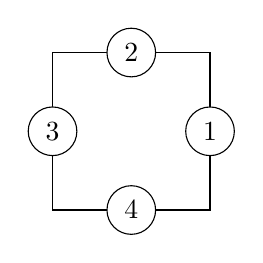
\begin{tikzpicture}
      \draw (0,0) rectangle (2,2);
      \node[draw, fill=white, circle] at (1,2) {2}; % top
      \node[draw, fill=white, circle] at (1,0) {4}; % bottom
      \node[draw, fill=white, circle] at (0,1) {3}; % left
      \node[draw, fill=white, circle] at (2,1) {1}; % right
      % \node[draw, rotate=0] at (1,1) {$D_8$}; % right
    \end{tikzpicture}
    ~
    \begin{tikzpicture}
      \draw (0,0) rectangle (2,2);
      \node[fill=white, circle] at (1,2) {3}; % top
      \node[fill=white, circle] at (1,0) {1}; % bottom
      \node[fill=white, circle] at (0,1) {4}; % left
      \node[fill=white, circle] at (2,1) {2}; % right
      % \node[draw, rotate=270] at (1,1) {$D_8$}; % right
    \end{tikzpicture}
    ~
    \begin{tikzpicture}
      \draw (0,0) rectangle (2,2);
      \node[fill=white, circle] at (1,2) {4}; % top
      \node[fill=white, circle] at (1,0) {2}; % bottom
      \node[fill=white, circle] at (0,1) {1}; % left
      \node[fill=white, circle] at (2,1) {3}; % right
      % \node[draw, rotate=180] at (1,1) {$D_8$}; % right
    \end{tikzpicture}
    ~
    \begin{tikzpicture}
      \draw (0,0) rectangle (2,2);
      \node[fill=white, circle] at (1,2) {1}; % top
      \node[fill=white, circle] at (1,0) {3}; % bottom
      \node[fill=white, circle] at (0,1) {2}; % left
      \node[fill=white, circle] at (2,1) {4}; % right
      % \node[draw, rotate=90] at (1,1) {$D_8$}; % right
    \end{tikzpicture}

    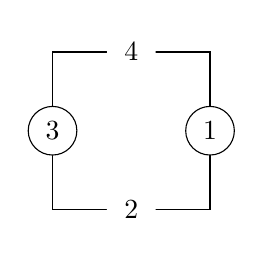
\begin{tikzpicture}
      \draw (0,0) rectangle (2,2);
      \node[fill=white, circle] at (1,0) {2}; % bottom
      \node[fill=white, circle] at (1,2) {4}; % top
      \node[draw, fill=white, circle] at (0,1) {3}; % left
      \node[draw, fill=white, circle] at (2,1) {1}; % right
      % \node[draw, yscale=-1] at (1,1) {$D_8$}; % right

    \end{tikzpicture}
    ~
    \begin{tikzpicture}
      \draw (0,0) rectangle (2,2);
      \node[fill=white, circle] at (1,0) {3}; % bottom
      \node[fill=white, circle] at (1,2) {1}; % top
      \node[fill=white, circle] at (0,1) {4}; % left
      \node[fill=white, circle] at (2,1) {2}; % right
      % \node[draw, yscale=-1, rotate=270] at (1,1) {$D_8$}; % right
    \end{tikzpicture}
    ~
    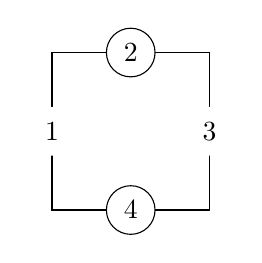
\begin{tikzpicture}
      \draw (0,0) rectangle (2,2);
      \node[draw, fill=white, circle] at (1,0) {4}; % bottom
      \node[draw, fill=white, circle] at (1,2) {2}; % top
      \node[fill=white, circle] at (0,1) {1}; % left
      \node[fill=white, circle] at (2,1) {3}; % right
      % \node[draw, yscale=-1, rotate=180] at (1,1) {$D_8$}; % right
    \end{tikzpicture}
    ~
    \begin{tikzpicture}
      \draw (0,0) rectangle (2,2);
      \node[fill=white, circle] at (1,0) {1}; % bottom
      \node[fill=white, circle] at (1,2) {3}; % top
      \node[fill=white, circle] at (0,1) {2}; % left
      \node[fill=white, circle] at (2,1) {4}; % right
      % \node[draw, yscale=-1, rotate=90] at (1,1) {$D_8$}; % right
    \end{tikzpicture}
    \caption[Facet derangements of a square.]{
      The $2^{2}2! = 8$ symmetries of a square with fixed sides circled.
      The square ($2$-dimensional hypercube) has symmetry group
      $S(2,2) = (\mathbb{Z}/2\mathbb{Z}) \wr \mathbb S_2$ and $D(2,2) = 5$ of these
      symmetries are derangements, meaning that they do not fix any sides.
    }
    \label{fig:squareDerangements}
  \end{figure}
\end{example}

While Theorem \ref{firstTheorem} gave us our first way to efficiently compute
the expected value of the first letter of a permutation on $kn$ letters with
a given number of $k$-cycles, we can also compute this efficiently with
Theorem \ref{secondTheorem} by using the formulas for $D(k,n)$ in Theorem \ref{derangementEGF}.
But this is not the only reason that Theorem \ref{secondTheorem} is of interest;
because of the structure of the formula it provides, this theorem suggests other
quantitative and qualitative insights.

Recall that when there are no restrictions on a permutation $\pi \in S_{kn}$, the
first letter is equally likely to take on any value,
so $\mathbb{E}[\pi(1) \mid \pi \in S_{kn}] = (kn+1)/2$.
% Recall also Proposition \ref{allSame},
% which stated that for $a \neq 1 \neq b$, there are the number of permutations with
% $m$ $k$-cycles starting with $a$ as there are starting with $b$.
The first insight given by Theorem \ref{secondTheorem}
is that the expected value of $\pi(1)$ given some
number of $k$ cycles differs from $(kn+1)/2$ by at most $1/2$,
because $D(k,N) \geq 1$ for $k \geq 2$.
%
Secondly, since $D(k, N)$ increases as a function of $N$, the expected value
gets closer to $(kn+1)/2$ as the number of $k$-cycles decreases.
%
Lastly, the numerator of $(-1)^{n-m}$ in the second summand of
Equation \ref{eq:main} shows that the expected value of the first letter is
larger than $(kn+1)/2$ if and only if $n$ and $m$ have the same parity.
% Together, Corollary \ref{cor:kNotDivideN} and Theorem \ref{secondTheorem} fully
% explain both the even- and odd-indexed rows in the table in
% Figure \ref{fig:twoCyclesTable}. Corollary \ref{cor:kNotDivideN} states that if
% $k \nmid n$, then $\pi(1)$ is equally likely to be any value between $1$ and $n$;
% Theorem \ref{secondTheorem} states that when $k \mid n$, then $\pi(1)$ is
% slightly more or less likely to be $1$, in an amount that relates to the number
% of derangements of a generalized symmetric group.

\section{A \texorpdfstring{$k$}{k}-cycle preserving bijection}
\label{section:bijection}
Motivated by Equation \ref{eq:bijectionDifference0}, this section describes a
family of bijections,
  \[\phi_k \colon S_{n-1} \times [n] \rightarrow S_n,\]
each of which preserves the number of $k$-cycles when $k \nmid n$.
Of course, there is no map that preserves the number of $k$-cycles when $k \mid n$. For example, a permutation in
$S_n$ consisting entirely of $k$-cycles contains $n/k$ $k$-cycles, while a permutation
in $S_{n-1}$ can contain at most $n/k - 1$ $k$-cycles by the pigeonhole principle.

% \begin{definition}
%   Given a word $\alpha = \alpha_1\alpha_2 \dots \alpha_n$ consisting of $n$
%   distinct letters in $\mathbb{N}_{>0}$, and a positive integer
%   $x \in \mathbb{N}_{>0}$, a \textbf{normalization} of the pair $(x,\alpha)$ is
%   a relabeling of the letters to be $[n+1]$, with each number appearing once,
%   where $\alpha$ keeps the same relative order.
% \end{definition}
% \begin{example}
%   The normalization of $(3,1398)$ is $\operatorname{normalize}(3,1376) = (2, 1354)$.
% \end{example}

Informally, these maps are defined by writing down a permutation $\sigma \in S_{n-1}$ in
\emph{canonical cycle notation}, incrementing all letters in $\sigma$
that are greater than or equal to $x \in [n]$,
inserting $x$ into the rightmost cycle, and then recursively moving letters into or out of subsequent cycles,
whenever a $k$-cycle is turned into a $(k+1)$-cycle or a $(k-1)$-cycle is
turned into a $k$-cycle.

\subsection{Example of recursive structure}

The definition of the map can look complicated, so it's worthwhile to start with
an example to give some sense of the overarching idea.

\begin{example}
  This example illustrates how the map $\phi_3$ inserts $I$ into
  the permutation $(D76)(E)(F32)(G91C)(K54)(LJ8)(MB)(NAH)$ while preserving the
  number of $3$-cycles.
  The maps $\phi_k$ and $\psi_k$ are the result of moving letters according
  to the arrows and are applied from right-to-left.
  (This example uses the convention that $1 < 2 < \dots < 9 < A < B < \dots < N$.)

  ~

  \begin{align*}
    &\phi_3(
      (D         7          6)
      (E                                          \nS{eEnd})
      (F         \nW{3}{3}  2                     \nS{2End})
      (G         \nW{9}{9}  1          \nW{C}{C})
      (K \nS{k5} 5          \nW{4}{4})
      (L \nS{lj} J          \nW{8}{8})
      (M \nS{mb} B                                \nS{bEnd})
      (N         \nW{A}{A}  H                     \nS{hEnd})
      ,
      \nW{I}{I}
    ) \\
    &\hspace{1cm} = (D76)(E3)(F29)(G1)(KC5)(L4J)(M8BA)(NHI)
  \end{align*}
  \begin{tikzpicture}[remember picture,overlay]
    \draw[thick, ->]  (I) to[out=90, in=90, looseness=3.4] node[midway, above]{$\phi_3$} (hEnd);
    \draw[thick, ->]  (A) to[out=90, in=90, looseness=2] node[midway, above]{$\phi_3$} (bEnd);
    \draw[thick, ->]  (8) to[out=90, in=90, looseness=2] node[midway, above]{$\psi_3$} (mb);
    \draw[thick, ->]  (4) to[out=90, in=90, looseness=2] node[midway, above]{$\psi_3$} (lj);
    \draw[thick, ->]  (C) to[out=90, in=90, looseness=2] node[midway, above]{$\psi_3$} (k5);
    \draw[thick, ->]  (9) to[out=90, in=90, looseness=2] node[midway, above]{$\phi_3$} (2End);
    \draw[thick, ->]  (3) to[out=90, in=90, looseness=2] node[midway, above]{$\phi_3$} (eEnd);
  \end{tikzpicture}

  \begin{align*}
    &\psi_3(
      (D         7         6)
      (E                   \nW{3}{3})
      (F \nS{f2} 2         \nW{9}{9})
      (G \nS{g1} 1                             \nS{1End})
      (K         \nW{C}{C} 5                   \nS{5End})
      (L         \nW{4}{4} J                   \nS{jEnd})
      (M         \nW{8}{8} B         \nW{A}{A})
      (N \nS{nh} H         \nW{I}{I})
    )\nS{outside}\\
    &\hspace{1cm} = ((D76)(E)(F32)(G91C)(K54)(LJ8)(MB)(NAH),I)
  \end{align*}
  \begin{tikzpicture}[remember picture,overlay]
    \draw[thick, ->]  (3) to[out=90, in=90, looseness=2] node[midway, above]{$\psi_3$} (f2);
    \draw[thick, ->]  (9) to[out=90, in=90, looseness=2] node[midway, above]{$\psi_3$} (g1);
    \draw[thick, ->]  (C) to[out=90, in=90, looseness=2] node[midway, above]{$\phi_3$} (1End);
    \draw[thick, ->]  (4) to[out=90, in=90, looseness=2] node[midway, above]{$\phi_3$} (5End);
    \draw[thick, ->]  (8) to[out=90, in=90, looseness=2] node[midway, above]{$\phi_3$} (jEnd);
    \draw[thick, ->]  (A) to[out=90, in=90, looseness=2] node[midway, above]{$\psi_3$} (nh);
    \draw[thick, ->]  (I) to[out=90, in=90, looseness=3.4] node[midway, above]{$\psi_3$} (outside);
  \end{tikzpicture}
\end{example}
Again, it is worth reemphasizing that the following definitions will follow the
convention that permutations are written in canonical cycle notation, \[
  \pi =
    \underbrace{(c^{(t)}_1\cdots c^{(t)}_{\ell_t})}_{c^{(t)}}
    \cdots
    \underbrace{(c^{(1)}_1\cdots c^{(1)}_{\ell_1})}_{c^{(1)}},
\] where cycle $c^{(i)} = (c^{(i)}_1 \cdots c^{(i)}_{\ell_i})$ has $\ell_i$ letters.
This means that the first letter in each cycle, $c^{(i)}_1$, is the largest letter in that cycle,
and that the cycles are ordered in increasing order by first letter when read from right-to-left:
$c^{(i+1)}_1 < c^{(i)}_1$ for all $i$.
\subsection{Formal definition and properties}
\begin{definition}
  Define
  $\phi_k \colon S_{n-1} \times [n] \mapsto S_{n}$ recursively as follows:
  \begin{equation}
    \phi_k(\emptyset, 1) = (1),
  \end{equation}
  and for $n>1$, $\pi \in S_{n-1}$, and $x \in [n]$,
  \begin{numcases}{\phi_k(\pi, x) =}
    \label{eq:phi_a}
    c^{(t)} \cdots c^{(1)}(x)                                                           & $x > c^{(1)}_1$            \\[10pt]
    \label{eq:phi_b}
    \phi_k(c^{(t)} \cdots c^{(2)}, c^{(1)}_2)(c^{(1)}_1 c^{(1)}_3 \cdots c^{(1)}_{k} x) & $\ell_1 = k$               \\[10pt]
    \label{eq:phi_c}
    \pi' (c^{(1)}_1 x' c^{(1)}_2\cdots c^{(1)}_{k-1} x)                                 & $\ell_1 = k-1, t > 1$ \\[10pt]
    \label{eq:phi_d}
    c^{(t)} \cdots c^{(2)} (c^{(1)}_1 \cdots c^{(1)}_{\ell_1} x)                        & otherwise.
  \end{numcases}
  Here, $\phi_k$ depends on the auxillary function
  $\psi_k \colon S_{n} \mapsto S_{n-1} \times [n]$,
  \begin{numcases}{\psi_k(\pi) =}
    \label{eq:psi_a}
    \left(c^{(t)} \dots c^{(2)}, c^{(1)}_1\right)                                                              & $\ell_1 = 1$             \\[10pt]
    \label{eq:psi_b}
    \left(\phi_k(c^{(t)} \cdots c^{(2)}, a_2^{(1)})(c^{(1)}_1 c^{(1)}_3 \dots c^{(1)}_k), c^{(1)}_{k+1}\right) & $\ell_1 = k + 1$         \\[10pt]
    \label{eq:psi_c}
    \left(\pi'(c^{(1)}_1 x' c^{(1)}_2 \dots c^{(1)}_{k-1}), c^{(1)}_k\right)                                   & $\ell_1 = k, t > 1$ \\[10pt]
    \label{eq:psi_d}
    \left(c^{(t)} \cdots c^{(2)}(c^{(1)}_1\cdots c^{(1)}_{\ell_1-1}),c^{(1)}_{\ell_1}\right)                   & otherwise,
  \end{numcases}
  and in both functions, $(\pi', x') = \psi(c^{(t)}\dots c^{(2)})$.
\end{definition}

\begin{note}
  Strictly speaking, $\phi_k$ and $\psi_k$ have an additional implicit
  parameter $n$, which indicates the size of permutation that these functions
  act on. Since the construction of these functions do not depend on $n$, this
  is suppressed in the notation.
\end{note}
The following theorem motivates this map,
and together with Lemma \ref{lem:bijection}, it implies Equation \ref{eq:bijectionDifference0}.
\begin{theorem}
  If $k \nmid n$, the number of $k$-cycles of $\pi \in S_{n-1}$ is equal to the number of $k$-cycles in
  $\phi_k(\pi,x)$.
\end{theorem}
\begin{proof}
  By construction, the maps $\phi_k$ and $\psi_k$ change the rightmost cycle
  into a (different) $k$-cycle if it was previously a $k$-cycle, and they
  change non-$k$-cycles into non-$k$-cycles, except for the case where there is
  one cycle remaining with length $k-1$ (in the case of $\phi$) or length $k$
  (in the case of $\psi$). These cases can only be achieved when $k \mid n$, by
  the following lemma.
\end{proof}
\begin{lemma}
  The number of letters in $\pi$ in (recursive) applications of $\phi_k$ and
  $\psi_k$ are of congruent to $n - 1 \bmod k$ and $n \bmod k$, respectively.
  Therefore, the only time that the input to $\phi_k$ can be a single cycle of
  length $k-1$ or the input to $\psi_k$ can be a single cycle of length $k$ is
  when $n \equiv 0\ (\bmod\ k)$.
\end{lemma}
\begin{proof}
  The proof proceeds by induction on the number of recursive iterations of
  $\phi_k$ and $\psi_k$. The base case is clear: on the first application of a
  map is always
  $\phi_k \colon S_{n-1} \times [n] \rightarrow S_n$, and the input permutation
  has $n-1$ letters by definition.

  Now, either we're finished, or we recurse
  (Equations \ref{eq:phi_b}, \ref{eq:phi_c}, \ref{eq:psi_b}, or \ref{eq:psi_c}),
  which we look at case-by-case.
  \begin{enumerate}[leftmargin=*, label={\textbf{Case \arabic*.}}]
    \item In Equation \ref{eq:phi_b}, the map $\phi_k$ sets aside $k$ letters from the input, so the number of letters in the recursive input to $\phi_k$ is also congruent to $n - 1 \bmod k$.
    \item In Equation \ref{eq:phi_c}, the map $\phi_k$ sets aside $k - 1$ letters from the leftmost cycle of the input. Since the number of letters in the original permutation was congruent to $n-1 \bmod k$, the number of letters in the permutation being input to $\psi_k$ is congruent to $n   \bmod k$.
    \item In Equation \ref{eq:psi_b}, the map $\psi_k$ sets aside $k + 1$ letters from the leftmost cycle of the input. Since the number of letters in the original permutation was congruent to $n   \bmod k$, the number of letters in the permutation being input to $\phi_k$ is congruent to $n-1 \bmod k$.
    \item In Equation \ref{eq:psi_c}, the map $\psi_k$ sets aside $k$ letters from the input, so the number of letters in the recursive input to $\psi_k$ is also congruent to $n \bmod k$.
  \end{enumerate}
\end{proof}
The following lemma provides a certain ``niceness'' property of the map,
which allows us to analyze it. In particular, all recursive inputs in both
$\phi_k$ and $\psi_k$ are written in canonical cycle notation.
\begin{lemma}
  The output of $\phi_k$ is in canonical cycle notation.
\end{lemma}
\begin{proof}
  % TODO: Strictly speaking, this should be an inductive argument similar to
  % the previous.
  Canonical cycle notation is preserved by construction.
  In particular, $\phi_k$ moves the first letter in any cycle, and
  Equation \ref{eq:phi_a} guards against inserting a number into a cycle that
  is bigger than the largest number already in the cycle.
  Similarly, $\psi_k$ only moves the first letter in the case of Equation
  \ref{eq:psi_a}, but in this case, the cycle only has one letter, so this is
  equivalent to deleting the cycle.
\end{proof}
\subsection{Inverting the bijection}
\begin{lemma}
  \label{lem:bijection}
  The maps
  $\phi_k \colon S_{n-1} \times [n] \rightarrow S_n$ and
  $\psi_k \colon S_n \rightarrow S_{n-1} \times [n]$ are inverse to one another.
\end{lemma}
\begin{proof}
  To prove this lemma, it suffices to show that $\psi_k \circ \phi_k = \operatorname{id}$
  by induction on the number of cycles of $\pi$. This will simultaneously prove
  that $\phi_k \circ \psi_k = \operatorname{id}$, because $S_{n-1} \times [n]$
  and $S_n$, both having $n!$ elements, have the same cardinality.

  When $\pi$ has no cycles, the base case is clear:
  $\psi_k(\phi_k(\emptyset, x)) = \psi_k((x)) = (\emptyset, x)$.

  Now there are five remaining cases to check, corresponding to each of the
  cases in the definition of $\phi_k(\pi, x)$
   \begin{enumerate}[leftmargin=*, label={\textbf{Case \arabic*.}}]
    \item Assume $x > c_1^{(1)}$, so that $\phi_k(\pi,x)$ is evaluated via Equation \ref{eq:phi_a}: \begin{align}
      \psi_k(\phi_k(\pi, x))
      &= \psi_k(c^{(t)}\cdots c^{(1)}(x)) \\
      &= (c^{(t)}\cdots c^{(1)},x) \\
      &= (\pi, x).
    \end{align}
    \item Assume $\ell_1 = k$, so that $\phi_k(\pi,x)$ is evaluated via Equation \ref{eq:phi_b}:\begin{align}
      \psi_k(\phi_k(\pi, x))
      &= \psi_k(\phi_k(c^{(t)} \cdots c^{(2)}, c^{(1)}_2)
      \underbrace{
        (c^{(1)}_1 c^{(1)}_3 \cdots c^{(1)}_{k} x)
      }_{\text{length } k}) \\
      &= (\pi'(c^{(1)}_1x'c^{(1)}_3 \dots c^{(1)}_k), x)
    \end{align}
    \item Assume $\ell_1 = k - 1$ and $t > 1$, so that $\phi_k(\pi,x)$ is evaluated via Equation \ref{eq:phi_c}:  \begin{align}
      \psi_k(\phi_k(\pi, x))
      &= \psi_k(\pi'
        \underbrace{
          (c^{(1)}_1 x' c^{(1)}_2\cdots c^{(1)}_{k-1} x)
        }_{\text{length } k + 1}
      )
    \end{align} where $(\pi', x') = \psi_k(c^{(t)} \dots c^{(2)})$.
    Therefore, this simplifies by Equation \ref{eq:psi_c}: \begin{align}
      \psi_k(\phi_k(\pi, x)) &= \left(
        \phi_k(\pi', x')
        (c^{(1)}_1 \cdots c^{(1)}_{k-1}),
        x
      \right) \\
      &= \Big(
        \underbrace{
          \phi_k(\psi_k(c^{(t)} \dots c^{(2)}))
        }_{c^{(t)} \dots c^{(2)}}
        \underbrace{
          (c^{(1)}_1 \cdots c^{(1)}_{k-1})
        }_{c^{(1)}},
        x
      \Big) \\
      &= (\pi, x),
    \end{align} because $\phi_k(\psi_k(c^{(t)} \dots c^{(2)})) = c^{(t)} \dots c^{(2)}$
    by the induction hypothesis on $t-1$ letters.
    \item Assume that $x > c_1^{(1)}$ and $\ell_1 \not\in \{k-1,k\}$, so that $\phi_k(\pi,x)$ is evaluated via Equation \ref{eq:phi_d}: \begin{align}
      \psi_k(\phi_k(\pi, x))
      &= \psi_k(c^{(t)} \cdots c^{(2)} (c^{(1)}_1 \cdots c^{(1)}_{\ell_1} x)) \\
      &= (c^{(t)}\cdots c^{(1)},x) \\
      &= (\pi, x).
    \end{align}
    \item Assume that $\ell_1 = k-1$ and $t = 1$, so that $\phi_k(\pi,x)$ is evaluated via Equation \ref{eq:phi_d}: \begin{align}
      \psi_k(\phi_k(\pi, x))
      &= \psi_k((c^{(1)}_1 \cdots c^{(1)}_{k-1  } x)) \\
      &= (c^{(1)},x) \\
      &= (\pi, x).
    \end{align}
  \end{enumerate}
\end{proof}
In this section we constructed a recursively-defined map and its inverse to
give a bijective proof that $C_k(n,m) = nC_k(n-1,m)$ when $k \nmid n$. This
is a novel, reversible algorithm for inserting a letters into a permutation
that preserves the number of $k$-cycles whenever possible.
\section{Further directions}
\label{section:furtherDirections}
In the introduction, we mentioned Conger's paper which analyzed how the number
of descents of a permutation affects the expected value of the first letter
of the permutation.
And similarly in the following sections, we looked at how the number of $k$-cycles
affects the expected value of the first letter of the permutation.
This section will principally look at the obvious generalization: given some
permutation statistic $\operatorname{stat}\colon S_n \rightarrow \mathbb Z$,
does the map \begin{equation}
  f(n,m) = \mathbb E[\pi(i) \mid \pi \in S_n, \operatorname{stat}(\pi)=m]
\end{equation} have any interesting structure?

But notice that the first letter of a permutation is itself a statistic, so
we can play a more general game. Given pairs of statistics
$(\operatorname{stat}_1, \operatorname{stat}_2)$, does the map
\begin{equation}
  g(n,m) = \mathbb E[\operatorname{stat}_1(\pi) \mid \pi \in S_n, \operatorname{stat}_2(\pi)=m]
\end{equation} have any interesting structure?

\subsection{FindStat database}
The result by Conger gives the expected value of $\pi(1)$ given
$\operatorname{des}(\pi)$, and this paper gave the expected value of
$\pi(1)$ given the number of $k$-cycles of $\pi$. Of course, it would be
interesting to do analogous analysis with other permutations. In particular,
the FindStat permutation statistics database \cite{FindStat} contains over
370 different permutation statistics, and many of these appear to have some
structure with respect to the expected value of the first letter of a
permutation.

\subsection{Mahonian statistics}
In particular, the family of Mahonian statistics may be fruitful to investigate.
Below, we have given conjectures about two: the major index and the inversion number.
Mahonian statistics are maps
$\operatorname{mah} \colon S_n \rightarrow \mathbb{N}_{\geq0}$ that are
equidistributed with the inversion number.\cite{Foata} That is, \[
  \#\{w \in S_n : \operatorname{mah}(w) = k\} =
  \#\{w \in S_n : \operatorname{inv}(w) = k\}.
\]
Naturally, all Mahonian statistics share the same generating function: \[
  \sum_{\sigma \in S_n} x^{\operatorname{mah}(\sigma)}
    = [n]_q!
    = \prod_{i=0}^{n-1}\sum_{j=0}^i(q^j).
\]

Because the expected value of the first letter is given by the weighted sum of
the permutations with $\operatorname{mah}(w) = k$ divided by the number of such
permutations, $\mathbb{E}[\pi(1)\, |\, \pi \in S_n, \operatorname{mah}(\pi) = k]$
has a denominator that is (a factor of) $M(n,k)$, the number of permutations
of $w \in S_n$ such that $\operatorname{inv}(w) = k$. For fixed $k$, these
satisfy a degree $k$ polynomial for all $n > k$. Notably, in the cases of
the major index and the inversion number, the numerators appear to satisfy
degree $k$ and degree $k-1$ polynomials respectively.

\begin{conjecture}
  For fixed $k$ and $n > k$, the expected value of the first letter of a
  permutation with a given number of inversions satisfies a rational function
  in $n$ given by \[
    \mathbb{E}[\pi(1)\, |\, \pi \in S_n, \operatorname{inv}(\pi) = k]
    = \frac{M(n+1,k)}{M(n,k)},
  \] where $M(n,k)$, as above, is the number of permutations $w \in S_n$ such
  that $\operatorname{inv}(w) = k$.
\end{conjecture}

\begin{conjecture}
  For fixed $k > 0$ and $n \geq k$,
  $\mathbb{E}[\pi(1)\, |\, \pi \in S_n, \operatorname{maj}(\pi) = k]$
  satisfies a rational function in $n$ that is $1/(k+1)$ times the quotient of a monic
  degree-$(k+1)$ polynomial by a monic degree-$k$ polynomial. Specifically,

  \begin{align}
    \mathbb{E}[\pi(1)\, |\, \pi \in S_n, \operatorname{maj}(\pi) = 1] &= \frac{1}{2}\left(\frac{n^2 + n - 2}{n-1}\right),
    \\[2mm]
    \mathbb{E}[\pi(1)\, |\, \pi \in S_n, \operatorname{maj}(\pi) = 2] &= \frac{1}{3}\left(\frac{n^3 - n - 6}{n^2 - n - 2}\right),
    \\[2mm]
    \mathbb{E}[\pi(1)\, |\, \pi \in S_n, \operatorname{maj}(\pi) = 3] &= \frac{1}{4}\left(\frac{n^4 + 6 n^3 - 13 n^2 - 18 n}{n^3 - 7n}\right),
    \text{ and}
    \\[2mm]
    \mathbb{E}[\pi(1)\, |\, \pi \in S_n, \operatorname{maj}(\pi) = 4] &= \frac{1}{5}\left(\frac{n^5 + 20 n^4 - 45 n^3 - 80 n^2 - 16 n}{n^4 + 2 n^3 - 13 n^2 - 14 n}\right).
    % % \mathbb{E}[\pi(1)\, |\, \pi \in S_n, \operatorname{maj}(\pi) = 5] &= \frac{1}{6}\left(\frac{n^6 + 51 n^5 + 85 n^4 - 195 n^3 - 806 n^2 - 1296 n}{n^5 + 10 n^4 + 15 n^3 - 70 n^2 - 196 n}\right).
  \end{align}
  Note that the denominator is given by an integer multiple of $M(n,k)$,
  a degree $k$ polynomial.
\end{conjecture}

\subsection{An elusive bijection}

  Let $F_k(n, m)$ be the number of elements of the generalized symmetric group
  $S(k,n) = (\mathbb{Z}/k\mathbb{Z}) \wr S_n$ with $m$ fixed points,
  and recall that $C_k(n,m)$ is the number of elements of $S_{kn}$ with $m$ $k$-cycles.
  Then for each pair of nonnegative integers $(\alpha, \beta)$
  with $\alpha, \beta \leq n$, then as Lemma \ref{lem:fixedPointsAndCycles} suggests,
  there exists a bijection of sets \begin{equation}
    C_k(n, \alpha) \times F_k(n, \beta) \rightarrow C_k(n, \beta) \times F_k(n, \alpha).
  \end{equation}
  This bijection has proven to be elusive to construct outside of the special
  cases where $n=1$ or $k=1$.
  Note that, the map cannot be a group automorphism of $S_{kn} \times S(k,n)$,
  because the identity of this group is in $C_k(n,0) \times F_k(n,n)$, so it
  cannot be preserved under this map.

  It would be especially interesting if there's a way to use the embedding of
  $(\mathbb{Z}/k\mathbb{Z}) \wr S_n$ into $S_{kn}$ as the centralizer of an
  element that is the product of $n$ disjoint $k$ cycles.

\documentclass[tikz]{standalone}
\usepackage{tikz}
\usepackage{amsmath}
\usetikzlibrary{decorations.pathreplacing}
\newcommand{\xy}[2]{({(#1) - (#2)/2}, {0.866*(#2)})}
\pgfmathsetmacro{\n}{9}
\pgfmathsetmacro{\a}{4}
\pgfmathsetmacro{\b}{5}
\pgfmathsetmacro{\c}{7}
\pgfmathsetmacro{\d}{9}
% \title{Proof without words: There are $\binom{n+2}{4}$ equilateral triangles
% with vertices in the size $n$ triangular grid.}
% \author{Peter Kagey}
% \date{}
\begin{document}
% \maketitle
% \noindent
% Suppose $0 \leq A < B < C < D \leq n+1$.

% \noindent
% (Illustrated for $n=10$, $A = 4$, $B = 5$, $C=8$, $D=10$.)

% \vspace{1cm}
\begin{tikzpicture}
  \foreach \a in {0,...,\n} {
    \foreach \b [
      evaluate={\x using \a - \b/2},
      evaluate={\y using {0.866*\b}},
    ]
    in {0,...,\a} {
      \fill[gray] (\x,\y) circle (0.1);
    }
  }
  \draw[thick, gray, dashed] \xy{0}{0} -- \xy{\n}{0} -- \xy{\n}{\n} -- cycle;
  % \draw[ultra thick, red, dotted] \xy31 -- \xy{\d-3}1 -- \xy{\d-3}6 -- cycle;
  \draw[ultra thick, red, dotted]
    \xy{\d-2}{\d-\c+\b-1} circle (0.2) % top \xy{\d-2}{\d-\c+\b-1}
    \xy{\d-2-0.2}{\d-\c+\b-1-0.2} -- % top left
    \xy{\d-\b-1}{\d-\c} -- % bottom left
    \xy{\d-2}{\d-\c} -- % bottom right
    \xy{\d-2}{\d-\c+\b-1-0.2} % top right
  ;
  \draw[fill=blue, fill opacity=0.5, line width=3]
    \xy{\d-\b+\a-2}{\d-\c} -- % bottom
    \xy{\d-2}{\d-\c+\a-1} --  % right
    \xy{\d-\b-1+\b-\a}{\d-\c+\b-\a} -- % left
    cycle
  ;
  \draw[ultra thick, decorate,decoration={brace,amplitude=10pt},xshift=0pt,yshift=-0.25cm]
    \xy{\d-2}{\d-\c} -- \xy{\d-\b-1}{\d-\c}
    node [rectangle,draw,fill=white,midway,anchor=north,xshift=0cm, yshift=-0.5cm] {$B$}
  ;
  \draw[ultra thick, decorate,decoration={brace,amplitude=10pt},xshift=0.2165cm,yshift=0.125cm]
    \xy{\d-2}{\d-\c+\a-1} -- \xy{\d-2}{\d-\c}
    node [rectangle,draw,fill=white,midway,anchor=west,xshift=0.433cm, yshift=0.25cm] {$A$}
  ;
  \draw[ultra thick, decorate,decoration={brace,amplitude=10pt},xshift=-0.2165cm,yshift=-0.125cm]
    \xy{\d-2}{\d-\c+\b-1} -- \xy{\d-2}{\d-2}
    node [rectangle,draw,fill=white,midway,anchor=east,xshift=-0.433cm, yshift=-0.25cm] {$C - B + 1$}
  ;
  \draw[ultra thick, decorate,decoration={brace,amplitude=10pt},xshift=0.2165cm,yshift=-0.125cm]
    \xy{\n}{\d-\c+\b-1+\n+2-\d} -- \xy{\d-2}{\d-\c+\b-1}
    node [rectangle,draw,fill=white,midway,anchor=west,xshift=0.433cm, yshift=-0.25cm] {$n + 3 - D$}
  ;
\end{tikzpicture}
\end{document}

\chapter{Unranking Restricted Permutations}
\label{cha:UnrankingMenage}
TODO

\section{TODO}
\begin{enumerate}
  \item Introduction
  \item Define \textbf{derived} complementary board $B_\alpha^c$?
  \item If we do a cyclic rotation of the rows of a chessboard, we get
    essentially the same thing.
  \item Move code to Appendix.
  \item Define $B_\alpha$ and $\overline{B}_\alpha^c$.
  \item Do we want to talk about parking functions?
  \item Is it worthwhile to discuss prefix functions for compositions, etc.?
  \item Make sure ``derank'' doesn't occur anywhere.
  \item Gives a way of sampling uniformly at random.
\end{enumerate}

% %%%%%%%%%%%%%%%%%%%%%%%%%%%%%%%%%%%%%%%%%%%%%
% Section 1
% %%%%%%%%%%%%%%%%%%%%%%%%%%%%%%%%%%%%%%%%%%%%%
\section{Overview and History}

In January 2020, Richard Arratia sent out an email announcing a talk he was
going to give on de-ranking derangements.

By January 2021, he announced a \$100 prize for solving the analogous problem
with m\'enage permutations. I solved that too.

Richard was interested in a more general question, which I found contagious:
Given some family of combinatorial objects that can be quickly counted
(say unlabelled simple graphs on $n$ vertices)
and some total ordering on them,
when is it possible to \textbf{unrank} the collection in some computationally
efficient way?

\begin{definition}
  Let $\mathcal C$ be a totally ordered finite set, and
  let $\{c_i\}_{i=1}^{|\mathcal C|}$ be the unique sequence of elements in
  $\mathcal{C}$ such that $c_i < c_{i+1}$ for all $1 \leq i < |\mathcal{C}|$.

  The \textbf{ranking map} is the map
  $\operatorname{rank}_{\mathcal{C}} \colon \mathcal{C} \rightarrow \mathbb N_{>0}$
  which sends $c_i \mapsto i$.

  The \textbf{unranking map} is the inverse map
  $\operatorname{unrank}_{\mathcal{C}} \colon \mathbb N_{>0} \rightarrow \mathcal{C}$
  which sends $i \mapsto c_i$.
\end{definition}

In abstract terms, these maps are not particularly interesting, but in practical
terms it can be quite difficult to efficiently compute a given ranking or
unranking from a given totally ordered set. After all, when these sets
grow in exponential time or worse, explicitly constructing the sequence and
doing a search is not computationally feasible.

In Appendix TODO, we will provide examples of total orders on combinatorial
objects $\mathcal{C}$ for which constructing efficient

% Of course, we can usually create an algorithm to give the $i$-th object without
% simply enumerating all of the objects explicitly? We want to ``jump in'' to a
% specific place on the list. Another interesting question:
% what if you get to supply both the total order and the unranking algorithm?

In this chapter we're going to explore that idea. We're going to show a general
theory that allows us to de-rank
permutations in lexicographic order,
derangements in lexicographic order,
partitions and compositions of $n$ in lexicographic order,
labeled trees by lexicographic order of Pr\"ufer code,
Lyndon words \cite{Kociumaka2014} (de Bruijn Sequences?),
Dyck path in lexicographic order?
% %%%%%%%%%%%%%%%%%%%%%%%%%%%%%%%%%%%%%%%%%%%%%
% Section 2
% %%%%%%%%%%%%%%%%%%%%%%%%%%%%%%%%%%%%%%%%%%%%%
\section{Prefix Counting and Word Ranking}

% If we can efficiently count how many objects in
% $[n]^k$ start with a given prefix
% (in $O(T(n,k))$ time),
% then we can just walk down the possible letters until
% we get to the right spot ($O(nkT(n,k))$).

\begin{lemma}
  If we have
  an efficient way to compute the unranking map,
  an efficient way to compare two elements in the total order,
  and an efficient way of computing the number of objects at hand, $|\mathcal C|$,
  then we can efficiently compute the ranking map.
  \label{lemma:unrankToRank}
\end{lemma}
\begin{proof}
  We can do a binary search. (TODO: write pseudo-code algorithm?)
\end{proof}

\subsection{Counting Words With a Given Prefix}
In both the case of unranking derangements and menage permutations
(and in many other applications) our combinatorial objects are
words and our total order is lexicographic order.

\begin{definition}
  \textbf{Lexicographic order} is a total ordering on words where $w < v$ ... TODO
\end{definition}

\begin{definition}
  A finite \textbf{word} $w$ over an alphabet $\mathcal A$ is a finite sequence
  $\{w_i \in \mathcal A\}_{i=1}^N$.

  The collection of finite words over the alphabet $\mathcal A$ is denoted by
  $\mathcal{W}_\mathcal{A}$, or just $\mathcal{W}$ when the alphabet is
  implicit from context.
\end{definition}

\begin{definition}
  A word $w = \{w_i \in \mathcal A\}_{i=1}^N$ is said to begin with a
  \textbf{prefix} $\alpha = \{\alpha_i \in \mathcal A\}_{i=1}^M$ if
  $M \leq N$ and $w_i = \alpha_i$ for all $i \leq M$.
\end{definition}

\begin{lemma}
  Let $\mathcal{W}$ be the set of words of any length on the alphabet $[n]$,
  and let $\mathcal C \subsetneq \mathcal{W}$ be a finite subset of words
  on this alphabet, with a total order equal to its lexicographic order.

  Then let
  $\#\operatorname{prefix}_{\mathcal C}\colon \mathcal{W} \rightarrow \mathcal{C}$
  be the function that counts the number of words in $\mathcal C$ that begin
  with a given prefix.

  Then the unranking function can be computed recursively by \[
    \operatorname{unrank}_\mathcal{C}(i) = f^{\mathcal C}_i((1), 0)
  \] where
  \begin{equation}
  f^{\mathcal C}_i(\alpha, j) = \begin{cases}
    \alpha
      & i \in (j, j + \#\operatorname{prefix}_\mathcal{C}(\alpha)] \text{ and } \alpha \in \mathcal{C} \\
    f^{\mathcal C}_i(\alpha', j)
      & i \in (j, j + \#\operatorname{prefix}_\mathcal{C}(\alpha)] \text{ and } \alpha \not\in \mathcal{C} \\
    f^{\mathcal C}_i(\alpha'', j + \#\operatorname{prefix}_\mathcal{C}(\alpha))
      & \text{otherwise},
  \end{cases}
\end{equation}
where
$\alpha = (\alpha_1, \alpha_2, \dots, \alpha_\ell)$,
$\alpha' = (\alpha_1, \alpha_2, \dots, \alpha_\ell, 1)$,
$\alpha'' = (\alpha_1, \alpha_2, \dots, \alpha_{\ell-1}, 1 + \alpha_\ell)$,
and $j$ denotes the number of words in $\mathcal{C}$ that occur strictly
before $\alpha$.
\end{lemma}
\begin{proof}
  TODO (sketch)
  The second line appends a letter, which can happen at most $n$ times.
  The third line increments the last letter, which can happen at most $k$ times
  per position.
\end{proof}

This shows that if we can construct a function
$\#\operatorname{prefix}_\mathcal{C}$ that efficiently counts the number of
elements of $\mathcal{C}$ with a given prefix, then we can efficiently rank and
unrank the elements of $\mathcal{C}$ in lexicographic order.
% This technique works when we can write our objects as a word in $[n]^k$, and
% we order the objects
% by the lexicographic order of the words. In the case that our objects cannot be
% written as words, or we are interested in an order other than lexicographic order,
% a different technique must be used.

\subsection{Ranking words}
In Lemma \ref{lemma:unrankToRank}, we showed that given an efficient algorithm
to compute $\operatorname{unrank}_\mathcal{C}$, we can derive an efficient
algorithm to compute $\operatorname{rank}_\mathcal{C}$, on the order of
$O(\log(|\mathcal{C}|\operatorname{unrank}_\mathcal{C}(n)))$
(TODO: make the size of the input explicit.)

However, we can provide a faster algorithm via another recursive function:
$\operatorname{rank}_\mathcal{C}(w) = g_w(1,1,0)$ where
\begin{equation}
  g_w(i, \ell, c) = \begin{cases}
    c + 1 & \ell = w_i \text{ and } i = |w| \\
    g_w(i + 1, 1, c) & \ell = w_i \text{ and } i < |w| \\
    g_w(i, \ell + 1, c + \#\operatorname{prefix}_\mathcal{C}(w')) & \ell < w_i,
  \end{cases}
\end{equation}
where $w' = (w_1, w_2, \dots, w_{i-1}, \ell)$.

\section{Basic Notions of Rook Theory}
Because we have showed that we can ... TODO
In the case of unranking derangements and permutations, it is useful to use
ideas from rook theory, which provides a theory for understanding
position-restricted permutations.
Rook Theory was introduced by Kaplansky and Riordan \cite{Kaplansky1946}
in their 1946 paper \textit{The Problem of the Rooks and its Applications}. In
it, they discuss problems of restricted permutations in the language of rooks
placed on a chessboard.

\begin{figure}
  \center
  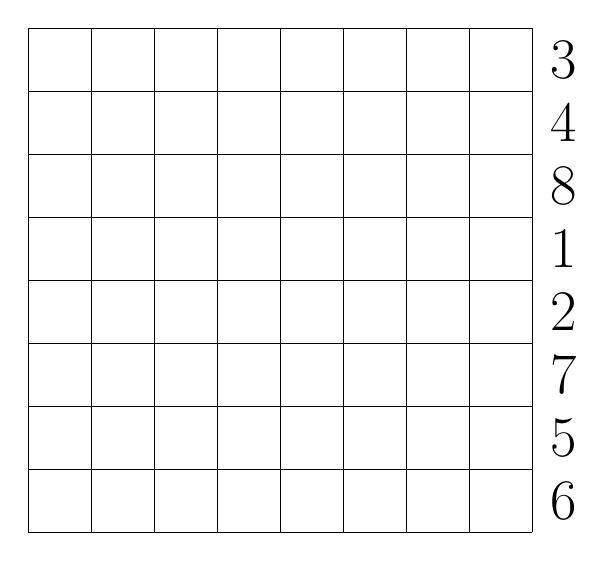
\begin{tikzpicture}[scale = 0.8]
    \foreach \i/\j in {1/3,2/4,3/8,4/1,5/2,6/7,7/5,8/6} {
      \node at (\j - 0.5, 8.5 - \i) {\huge\symrook};
      \node at (8.5, 8.5-\i) {\huge\j};
    }
    \draw (0,0) grid (8,8);
  \end{tikzpicture}
  \caption[A permutation corresponding to a rook placement.]{
    An illustration of the rook placement corresponding to the permutation
    $34812756 \in S_8$. A rook is placed in square $(i, \pi(i))$ for each $i$.
  }
  \label{fig:permutationFromRooks}
\end{figure}


\subsection{Definitions in rook theory}
We begin by introducing some preliminary ideas from rook theory.

\begin{definition}
  A \textit{board} $B$ is a subset of $[n] \times [n]$ which represents the
  squares of a $n \times n$ chessboard that rooks are allowed to be placed on.
  Every board $B$ has a \textit{complementary board}
  $B^c = ([n] \times [n]) \setminus B$, which consists of all of the
  squares of $B$ that a rook cannot be placed on.
\end{definition}

To each board, we can associate a generating polynomial that keeps track of the
number of ways to place a given number of rooks on the valid squares in such a
way that no two rooks are in the same row or column.

\begin{definition}
  The \textit{rook polynomial} associated with a board $B$,
  \[
    p_B(x) = r_0 + r_1 x + r_2 x^2 + \dots + r_n x^n,
  \]
  is a generating polynomial where $r_k$ denotes the number of $k$-element subsets
  of $B$ such that no two elements share an $x$-coordinate or a $y$-coordinate.
\end{definition}

In the context of permutations, we're typically interested in $r_n$, the number
of ways to place $n$ rooks on a restricted $n \times n$ board.
However, it turns out that a naive application of the techniques from
rook theory do not immediately allow us to count the number of
restricted permutations with a given prefix.
Computing the number of such permutations is known to be computationally hard
for a board with arbitrary restrictions.
We can see this by encoding a board $B$ as a $(0,1)$-matrix and computing the matrix
permanent. (In fact, Shevelev \cite{Shevelev1992} claims that
``the theory of enumerating the permutations with restricted positions
stimulated the development of the theory of the permanent.'')

\begin{lemma}
  Let $M_B = \{a_{ij}\}$ be an $n \times n$ matrix where \[
    a_{ij} = \begin{cases}
      1 & (i,j) \in B \\
      0 & (i,j) \not\in B
    \end{cases}.
  \]
  Then the coefficient of $x^n$ in $p_B(x)$ is given by the matrix permanent
  \[
    \operatorname{perm}(M_B) = \sum_{\sigma \in S_n} \prod_{i=1}^n a_{i\sigma(i)}.
  \]
\end{lemma}

Now is an appropriate time to recall Valiant's Theorem.

\begin{theorem}[Valiant's Theorem \cite{Valiant1979}]
  Computing the permanent of a (0,1)-matrix is \#P-complete.
\end{theorem}

\begin{corollary}
  Computing the number of rook placements on an arbitrary $n \times n$ board is
  \#P-hard.
\end{corollary}

Therefore, in order to compute the number of permutations, we must exploit some
additional structure of the restrictions.

\subsection{Techniques of Rook Theory}
Rook polynomials can be computed recursively. The base case is that
for an empty board $B = \emptyset$, the corresponding rook polynomial is
$p_\emptyset(x) = 1$, because there is one way to place no rooks, and no way
to place one or more rooks.
\begin{lemma}[\cite{Riordan1980}]
  Given a board, $B$, then for any square $(x,y) \in B$, we can define
  the resulting boards if we include or exclude the square respectively
  \begin{align}
    B_i &= \{(x',y') \in B : x \neq x' \text{ and } y \neq y'\} \\
    B_e &= B \setminus {(x,y)}.
  \end{align}
  Then we can write the rook polynomial for $B$ in terms of this decomposition.
  \[
    p_B(x) = xp_{B_i}(x) + p_{B_e}(x).
  \]
  \label{lemma:rookPolynomialRecursion}
\end{lemma}

If we want to compute a rook polynomial using this construction, we can end
up adding up lots of smaller rook polynomials---a number that is exponential in
the size of $B$.
However, when the number of squares in $B^c$ is small in some sense, it can be
easier to compute the rook polynomial $p_{B^c}$ and use the principle of
inclusion/exclusion on it's coefficients to determine the rook polynomial for
the original board, $B$.

In the case of derangements and m\'enage permutations, this is the strategy
we'll use.
Start by finding the resulting board from a given prefix,
find the rook polynomial of the complementary board, and
use the principle of inclusion/exclusion to determine the number of ways to
place rooks in the resulting board.

\section{Unranking Derangements}

In January 2020, Richard Arratia sent out an email proposing a seminar talk.
The title describes the first ``\$100 problem'':
\begin{problem}
``For $100$ dollars, what is the $500$ quadrillion-th derangement on $n=20$?''
\end{problem}

\begin{answer}
The computer program in Appendix TODO computed the answer in less than ten
milliseconds. When written as words in lexicographic order, the
derangement in $S_{20}$ with rank $5 \times 10^{17}$ is \[
  12\ 14\ 2\ 9\ 13\ 20\ 6\ 3\ 1\ 17\ 5\ 11\ 19\ 15\ 10\ 18\ 8\ 7\ 4\ 16.
\]
\end{answer}

Arratia's question focused on unranking derangements where the rank was
based on the total ordering that comes from writing the
permutations as words in lexicographic order.
Other authors have looked at unranking derangements based on other total
orderings. In particular, Mikawa and Tanaka \cite{Mikawa2014} give an algorithm
to rank/unrank derangements
with respect to \textit{lexicographic ordering in cycle notation}.

In this section we will develop an algorithm for ranking and unranking with
respect to their lexicographic ordering as words. The technique that we use will
broadly be re-used in the next section.
It is worthwhile to begin by recalling the definition of a derangement.
\begin{definition}
  A \textit{derangement} is a permutation $\pi \in S_n$ such that $\pi$ has no
  fixed points. That is, the set of derangements is \[
    \{\pi \in S_n : \pi(i) \neq i\ \forall i \in [n]\}.
  \]
\end{definition}

\subsection{The complementary board.}
In order to compute the number of derangements with a given prefix, it is
useful to look at the board that results after placing $k$ rooks according to
these positions, as illustrated in Figure \ref{fig:derangementPrefix}.

\begin{figure}
  \center
  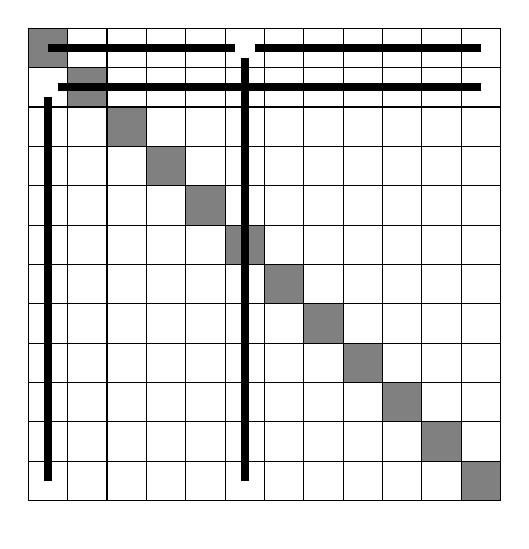
\begin{tikzpicture}[scale = 0.5]
    \path (0,-0.5) -- (0,6.5);
    \foreach \i in {0,...,11} { \fill[gray] (\i, 12-\i) rectangle (\i + 1, 11 - \i); }
    \draw (0,0) grid (12,12);
    \node (R1) at (5.5, 11.5) {\Large\rook};
    \node (R2) at (0.5, 10.5) {\Large\rook};
    \draw[line width = 3]
      (0.5,11.5) -- (R1) -- (11.5,11.5)
      (R1) -- (5.5,0.5)
    ;
    \draw[line width = 3]
      (R2) -- (11.5,10.5)
      (R2) -- (0.5,0.5)
    ;
  \end{tikzpicture}
  ~~
  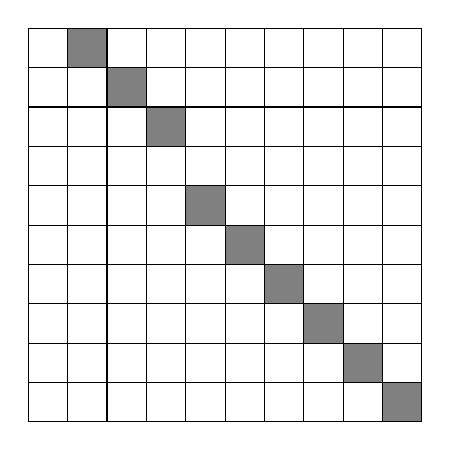
\begin{tikzpicture}[scale = 0.5]
    \path (0,-0.5) -- (0,6.5);
    \foreach \i in {1,...,3} { \fill[gray] (\i, 11-\i) rectangle (\i + 1, 10 - \i); }
    \foreach \i in {4,...,9} { \fill[gray] (\i, 10-\i) rectangle (\i + 1, 9 - \i); }
    \draw (0,0) grid (10,10);
  \end{tikzpicture}
  \caption[The derived board for a prefix of a derangement.]{An example of a prefix $\alpha = (6, 1)$, and the board that results
  from deleting the first $\ell = 2$ rows and columns $6$ and $1$.
  The derived complementary board of $B$ from $\alpha$ is
  $B^c_\alpha = \{(1,2), (2,3), (3,4), (5,5), \dots, (10,10)\}$.}
\label{fig:derangementPrefix}
\end{figure}


\begin{definition}
  If $B$ is an $n \times n$ board, and
  $\alpha = (\alpha_1, \alpha_2, \dots, \alpha_\ell)$ is a valid prefix of length
  $\ell$, then \textbf{derived complementary board} of $B$ from $\alpha$,
  denoted $B^c_\alpha$,
  is $B$ with the appropriate rows and columns removed and reindexed in such
  a way that $B^c_\alpha \subseteq [n - \ell] \times [n - \ell]$.
  % \[
  %   B^c_\alpha \cup \{(x, y) : x \in [n], y \in [\ell]\} \cup \{(x, y) : x \in \alpha, y \in [n]\}
  % \]
  % the \textit{derived complementary board} of $B$ from $\alpha$, denoted
  % $B^c_\alpha \subset [n-k]^2$ consisting of a subset of $B^c$, relabeled to
  % reflect ... TODO
\end{definition}
\begin{lemma}
  Given a valid $\ell$ letter prefix $(\alpha_1, \alpha_2, \dots, \alpha_\ell)$
  of a word on $n$ letters,
  the number of squares in the resulting complementary board is \[
    |B_\alpha^c| = n - \ell - |\{\ell+1, \ell+2, \dots, n\} \cap \{\alpha_1, \alpha_2, \dots, \alpha_\ell\}|,
  \] and no two of these squares are in the same row or column.
\end{lemma}
\begin{proof}
  TODO
  % Recall that $B^c = \{(1,1), (2,2), \dots, (n,n)\}$, so no square shares its
  % first or second coordinate with another square.
  % Because $B^c_\alpha$ is the result of deleting and relabeling the squares of
  % $B^c$, $B^c_\alpha$ also has two squares with with same first or second
  % coordinate.
  % In order to
  % Because the prefix is of length $\ell$, all of the squares in $B_\alpha^c$ must
  % have a first coordinate greater than $\ell$, that is,
  % $B_\alpha^c \subseteq \{(\ell+1, \ell+1), (\ell+2, \ell+2), \dots, (n, n)\}$.
  % Then, we can count how many of these remaining squares are in the same row or
  % column as a rook in the prefix. This number is the size of the intersection
  % $|\{\ell+1, \ell+2, \dots, N\} \cap \{\alpha_1, \alpha_2, \dots, \alpha_p\}|$.
\end{proof}

\subsection{Derangements with a given prefix}
Now that we have a way of quickly computing $|B_\alpha^c|$, we can compute the
number of ways to place $j$ rooks on the complementary board. We can use this
to compute the number of derangements that begin with the prefix $\alpha$.

\begin{lemma}
  The rook polynomial for the complementary board $B_\alpha^c$ is \begin{equation}
    p_{B_\alpha^c}(x) = \sum_{j = 0}^{|B_\alpha^c|} \binom{|B_\alpha^c|}{j}x^j.
  \end{equation}
\end{lemma}
\begin{proof}
  No two squares in $B^c$ (and thus $B^c_\alpha$) are in the same row or column.
  Thus the number of ways to place $j$ rooks is equivalent to selecting $j$
  cells from $|B^c_\alpha|$.
\end{proof}

Now we introduce a lemma of Stanley \cite{Stanley2011EC1} to compute the number
of TODO from a complementary board.

\begin{lemma}[\cite{Stanley2011EC1}]
  The number of ways, $N_0$, of placing $n$ nonattacking rooks on a board
  $B \subseteq [n] \times [n]$ is given by \[
    N_0 = \sum_{k=0}^n (-1)^k r_k (n-k)!,
  \] where $P_{B^c}(x) = \sum_{k=0}^n r_k x^k$.
  \label{lemma:CountsFromComplementaryPolynomials}
\end{lemma}

\begin{corollary}
  The number of derangements with prefix
  $\alpha = (\alpha_1, \alpha_2, \dots, \alpha_\ell)$
  is given by \[
    \#\operatorname{prefix}(\alpha)
    = \sum_{j=0}^{|B_\alpha^c|} (-1)^j \binom{|B_\alpha^c|}{j}(n-\ell-j)!,
  \] which is $\operatorname{A047920}(n-\ell, |B_\alpha^c|)$ in
  the On-Line Encyclopedia of Integer Sequences \cite{oeis}.
\end{corollary}

\begin{example}
  For example, for $N = 14$, we wish to count the number of derangements that
  start with the prefix $6\,1$. Since the prefix has two letters, $p = 2$ and
  $n = 14 - 2 = 12$. The only crossed-out cell that is deleted by the prefix in the
  remaining board is the cell that was in position $6$:
  in particular, $\{3,4,\dots,14\} \cap \{6, 1\} = 6$.
  Thus $k = 12 - 1 = 11$.
  Thus there are $A047920(12,11) = 190\,899\,411$ derangements that start
  with $6\,1$.
\end{example}
\begin{table}
\begin{tabular}{|l|r|l|c|l|}
  \hline
  $\alpha$ (prefix)   & $\operatorname{\#prefix}(\alpha)$ & index range & $|B_\alpha^c|$ & $f^{\mathcal{D}}_i(\alpha, \ell)$ \\
  \hline
  $1       $ & $0$    & $(0,0]$           & $-$ & $f^{\mathcal{D}}_{1000}(1, 0)$          \\
  $2       $ & $2119$ & $(0,2119]$        & $6$ & $f^{\mathcal{D}}_{1000}(2, 0)$          \\
  \hline
  $21      $ & $265$  & $(0, 265]$        & $6$ & $f^{\mathcal{D}}_{1000}(21, 0)$         \\
  $22      $ & $0$    & $(265, 265]$      & $-$ & $f^{\mathcal{D}}_{1000}(22, 265)$       \\
  $23      $ & $309$  & $(265, 574]$      & $5$ & $f^{\mathcal{D}}_{1000}(23, 265)$       \\
  $24      $ & $309$  & $(574, 883]$      & $5$ & $f^{\mathcal{D}}_{1000}(24, 574)$       \\
  $25      $ & $309$  & $(883, 1192]$     & $5$ & $f^{\mathcal{D}}_{1000}(25, 883)$       \\
  \hline
  $251     $ & $53$   & $(883, 936]$      & $4$ & $f^{\mathcal{D}}_{1000}(251, 883)$      \\
  $253     $ & $0$    & $(936, 936]$      & $-$ & $f^{\mathcal{D}}_{1000}(253, 936)$      \\
  $254     $ & $64$   & $(936, 1000]$     & $3$ & $f^{\mathcal{D}}_{1000}(254, 936)$      \\
  \hline
  $2541    $ & $11$   & $(936, 947]$      & $3$ & $f^{\mathcal{D}}_{1000}(2541, 936)$     \\
  $2543    $ & $11$   & $(947, 958]$      & $3$ & $f^{\mathcal{D}}_{1000}(2543, 947)$     \\
  $2546    $ & $14$   & $(958, 972]$      & $2$ & $f^{\mathcal{D}}_{1000}(2546, 958)$     \\
  $2547    $ & $14$   & $(972, 986]$      & $2$ & $f^{\mathcal{D}}_{1000}(2547, 972)$     \\
  $2548    $ & $14$   & $(986, 1000]$     & $2$ & $f^{\mathcal{D}}_{1000}(2548, 986)$     \\
  \hline
  $25481   $ & $3$    & $(986, 989]$      & $2$ & $f^{\mathcal{D}}_{1000}(25481, 986)$    \\
  $25483   $ & $3$    & $(989, 992]$      & $2$ & $f^{\mathcal{D}}_{1000}(25483, 989)$    \\
  $25486   $ & $4$    & $(992, 996]$      & $1$ & $f^{\mathcal{D}}_{1000}(25486, 992)$    \\
  $25487   $ & $4$    & $(996, 1000]$     & $1$ & $f^{\mathcal{D}}_{1000}(25487, 996)$    \\
  \hline
  $254871   $ & $2$   & $(996, 998]$      & $0$ & $f^{\mathcal{D}}_{1000}(254871, 996)$   \\
  $254873   $ & $2$   & $(998, 1000]$     & $0$ & $f^{\mathcal{D}}_{1000}(254873, 998)$   \\
  \hline
  $2548731  $ & $1$   & $(998, 999]$      & $0$ & $f^{\mathcal{D}}_{1000}(2548731, 998)$  \\
  $2548736  $ & $1$   & $(999, 1000]$     & $0$ & $f^{\mathcal{D}}_{1000}(2548736, 999)$  \\
  \hline
  $25487361 $ & $1$   & $(999, 1000]$     & $0$ & $f^{\mathcal{D}}_{1000}(25487361, 999)$ \\
  \hline
\end{tabular}
\caption[Steps for computing the $1000$th derangement in $S_8$]{
  There are $A000166(8) = 14833$ derangements on $8$ letters.
  This algorithm finds the derangement at index $1000$.
}
\end{table}

% %%%%%%%%%%%%%%%%%%%%%%%%%%%%%%%%%%%%%%%%%%%%%
% Section 3
% %%%%%%%%%%%%%%%%%%%%%%%%%%%%%%%%%%%%%%%%%%%%%
\section{Unranking M\'enage Permutations}

\subsection{Proof of concept (The \$100 answer!)}
In February 2020, Richard Arratia offered
\begin{problem}
  For $n=20$ there are $A000179(20) = 312\,400\,218\,671\,253\,762 > 3.1\cdot 10^{17}$
  m\'enage permutations.
  Determine the $10^{17}$-th such permutation when listed in lexicographic order.
\end{problem}
\begin{answer}
  The desired permutation is \begin{equation}
    7\ 16\ 19\ 12\ 2\ 8\ 15\ 1\ 18\ 14\ 3\ 9\ 20\ 10\ 5\ 17\ 13\ 4\ 11\ 6.
  \end{equation}
\end{answer}

A M\'enage permutation comes from the \textit{problème des ménages}. % https://en.wikipedia.org/wiki/M%C3%A9nage_problem
Here we will define it as
\begin{definition}
  A \textit{m\'enage permutation} is a permutation $\pi \in S_n$ such that for
  all $i \in [n]$,
  $\pi(i) \neq i$ and
  $\pi(i) + 1 \not\equiv i \bmod n$.
\end{definition}

We can use the prefix to get a new board, which is block diagonal
(whenever the prefix is non-empty), if we know the number of cells in each
block, we can compute the number of valid boards. This gives us the number of
m\'enage permutations with a given prefix.

Prefix $\Rightarrow$ grouped columns $\Rightarrow$ partition/multiset $\Rightarrow$ complementary polynomial $\Rightarrow$ count

\subsection{Block diagonal decomposition}
When we look at Figure TODO, it appears that placing rooks according to a prefix
results in a derived complementary board where the squares can be grouped into
sub-boards that don't share any rows or columns. We will see that this property
holds more generally, and we can exploit this in order to describe the number
of m\'enage permutations with a given prefix.

It is useful to begin by formalizing this notion of grouping squares.
\begin{definition}
  Two boards $B$ and $B'$ are called \textbf{disjoint} if no squares of $B$ are
  in the same row or column as any square in $B'$.
\end{definition}

The reason that we care about decomposing a board into disjoint parts
is because that perspective allows us to factor the rook polynomial.
\begin{lemma}[\cite{Kaplansky1946}]
  If $B$ can be partitioned into disjoint boards $b_1, b_2, \dots, b_m$,
  then the rook polynomial of $B$ is the product of the rook polynomials of
  the $b_i$s \[
    p_B(x) = \prod_{i=1}^m p_{b_i}(x).
  \]
\end{lemma}

The key insight is that after placing rooks in valid positions in
the top $1 \leq k \leq n-1$ rows, we get block-diagonal boards,
with three possible shapes, shown in Figure \ref{fig:blockShape}.
\begin{lemma}
  For $\ell \geq 1$, and prefix $\alpha = (\alpha_1, \alpha_2, \dots, \alpha_\ell)$
  the derived complementary board $B_\alpha^c$ can be partitioned into boards
  of one of four shapes.
  \begin{alignat*}{2}
    A_n      &= \{(i,i) : i \in [n]\}   &\cup\ \{(i,i+1) : i \in [n-1]\} \\ % (TODO Figure \ref{fig:blockShape}, left)
    A^\top_n &= \{(i,i) : i \in [n]\}   &\cup\ \{(i+1,i) : i \in [n-1]\} \\ % (TODO Figure \ref{fig:blockShape}, middle)
    B_n      &= \{(i,i) : i \in [n-1]\}\ &\cup\ \{(i+1,i) : i \in [n-1]\} \\ % (TODO Figure \ref{fig:blockShape}, right)
    B^\top_n &= \{(i,i) : i \in [n-1]\}\ &\cup\ \{(i,i+1) : i \in [n-1]\} % (TODO Figure \ref{fig:blockShape}, right)
  \end{alignat*}
\end{lemma}
\begin{proof}
  The proof proceeds by induction on the length of the prefix.

  To establish the base case, consider a prefix of length $1$.
  Because of the m\'enage restriction,
  $\alpha_1 \in \{2, 3, \dots, n-1\}$.
  It is quick to check that the resulting board is split into a part of shape
  $A_{\pi(1) - 1}$ and $A^\top_{n - \pi(1)}$.

  Now, assume that all blocks have shape $A_{n_1}$, $A^\top_{n_2}$,
  $B_{n_3}$ or $B^\top_{n_4}$. Placing a rook can remove a top row or a column
  or both in a given block. We will go block-by-block and consider each
  possibility.

  \begin{table}
    \begin{tabular}{|l|l|l|l|l|}
    \hline
    Rook placement & $A_n$ & $A^\top_n$ & $B_n$ & $B^\top_n$ \\
    \hline
    Top row                & x    & x              & x & x \\
    Column $i$             & x    & x              & x & x \\
    Top row and column $i$ & x    & x              & x & x \\
    \hline
    \end{tabular}
  \end{table}
  \begin{enumerate}
    \item $A_n      \rightarrow A_{n-1}$
    \item $A^\top_n \rightarrow B^\top_{n}$
    \item $B_n      \rightarrow A_{n-1}$
    \item $B^\top_n \rightarrow B^\top_{n}$
  \end{enumerate}

  The $i$-th column: \begin{enumerate}
    \item $A_n      \rightarrow (A_{i-1}, B_{n-i})$
    \item $A^\top_n \rightarrow (B_i,     A^\top_{n-i})$
    \item $B_n      \rightarrow (B_i,     B_{n-i})$
    \item $B^\top_n \rightarrow (A_{i-1}, B^\top_{n-i})$
  \end{enumerate}

  The top row and $i$-th column: \begin{enumerate}
    \item $A_n      \rightarrow (A_{i-2}, B_{n-i})$
    \item $A^\top_n \rightarrow (A_{i-1}, A^\top_{n-i})$
    \item $B_n      \rightarrow (A_{i-1}, B_{n-i})$
    \item $B^\top_n \rightarrow (A_{i-2}, B^\top_{n-i})$
  \end{enumerate}

  Of course, if neither a row or column is deleted, each board goes to itself.
\end{proof}

\begin{figure}[ht!]
  \center
  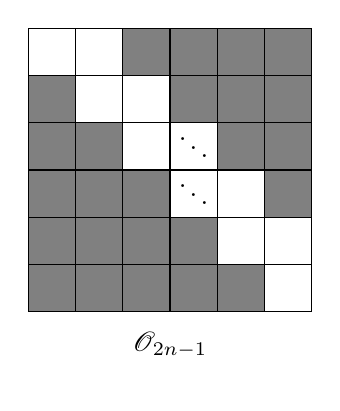
\begin{tikzpicture}[scale=0.6]
    \fill[gray] (1,0) rectangle (7,6);
    \foreach \i/\j in {1/5, 2/5, 2/4, 3/4, 3/3, 4/3, 4/2, 5/2, 5/1, 6/1, 6/0} { \fill[white] (\i, \j) rectangle (\i + 1, \j + 1); }
    \node at (4.5,3.65) {$\ddots$};
    \node at (4.5,2.65) {$\ddots$};
    \draw (1,0) grid (7,6);
    \path (1,-1.5) rectangle (7,6);
    \node at (4, -0.7) {$\mathcal{O}_{2n-1}$};
  \end{tikzpicture}
  ~
  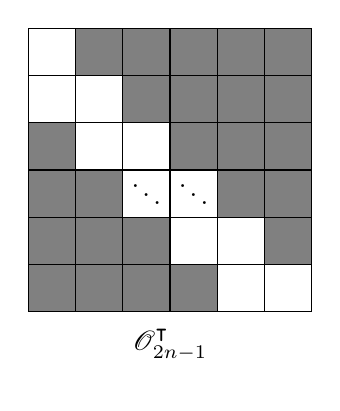
\begin{tikzpicture}[scale=0.6]
    \fill[gray] (1,0) rectangle (7,6);
    \foreach \i/\j in {1/5, 1/4, 2/4, 2/3, 3/2, 3/3, 4/1, 4/2, 5/1, 5/0, 6/0} { \fill[white] (\i, \j) rectangle (\i + 1, \j + 1); }
    \node at (3.5,2.65) {$\ddots$};
    \node at (4.5,2.65) {$\ddots$};
    \draw (1,0) grid (7,6);
    \path (1,-1.5) rectangle (7,6);
    \node at (4, -0.7) {$\mathcal{O}_{2n-1}^\intercal$};
  \end{tikzpicture}
  ~
  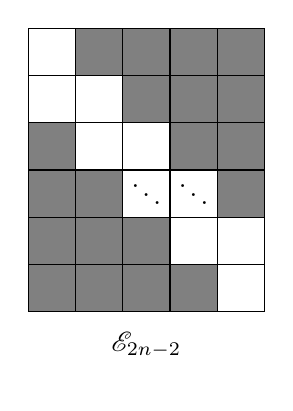
\begin{tikzpicture}[scale=0.6]
    \fill[gray] (1,0) rectangle (6,6);
    \foreach \i/\j in {1/4, 1/5, 2/3, 2/4, 3/2, 3/3, 4/1, 4/2, 5/0, 5/1} { \fill[white] (\i, \j) rectangle (\i + 1, \j + 1); }
    \node at (3.5,2.65) {$\ddots$};
    \node at (4.5,2.65) {$\ddots$};
    \draw (1,0) grid (6,6);
    \path (1,-1.5) rectangle (6,6);
    \node at (3.5, -0.7) {$\mathcal{E}_{2n-2}$};
  \end{tikzpicture}
  ~
  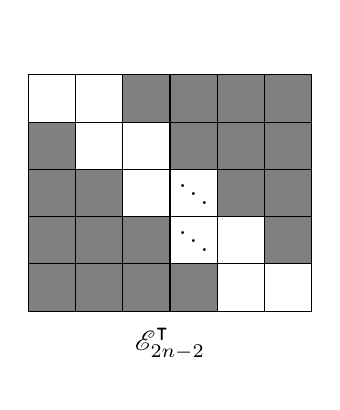
\begin{tikzpicture}[scale=0.6]
    \fill[gray] (1,1) rectangle (7,6);
    \foreach \i/\j in {1/5, 2/5, 2/4, 3/4, 3/3, 4/3, 4/2, 5/2, 5/1, 6/1} { \fill[white] (\i, \j) rectangle (\i + 1, \j + 1); }
    \node at (4.5,3.65) {$\ddots$};
    \node at (4.5,2.65) {$\ddots$};
    \path (1,-0.5) rectangle (7,7);
    \draw (1,1) grid (7,6);
    \node at (4, 0.3) {$\mathcal{E}_{2n-2}^\intercal$};
  \end{tikzpicture}
  \caption[Block shapes for a m\'enage permutation.]{
    Examples of each of the four staircase-shaped boards.
    The first two boards are on grids of size $n \times n$,
    the third is on a grid of size $n \times (n-1)$ and the
    fourth is on a grid of size $(n-1) \times n$.
  }
  \label{fig:blockShape}
\end{figure}

\begin{figure}[ht!]
  \center
  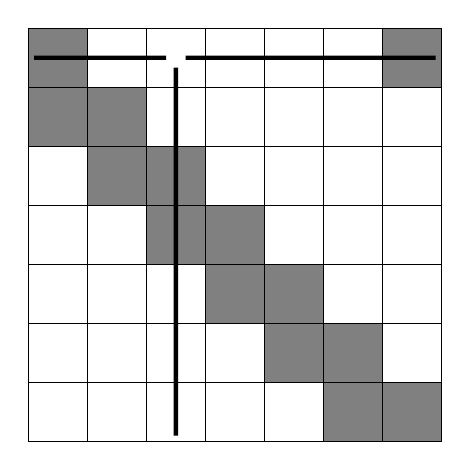
\begin{tikzpicture}[scale = 0.75]
    \foreach \i in {0,...,6} { \fill[gray] (\i, 6 - \i) rectangle (\i + 1, 7 - \i); }
    \foreach \i in {1,...,6} { \fill[gray] (\i-1, 6 - \i) rectangle (\i, 7 - \i); }
    \fill[gray] (6, 6) rectangle (7, 7);
    \draw (0,0) grid (7,7);
    \node (R) at (2.5, 6.5) {\huge\rook};
    \draw[ultra thick]
      (0.1,6.5) -- (R) -- (6.9,6.5)
      (R) -- (2.5,0.1)
    ;
  \end{tikzpicture}
  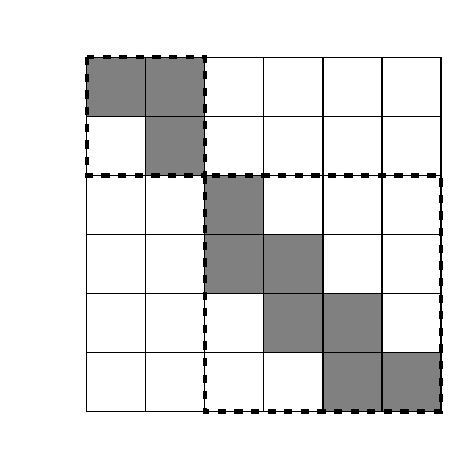
\begin{tikzpicture}[scale = 0.75]
    \path (0,-0.5) -- (0,6.5); % vertically center.
    \foreach \i/\j in {1/5, 2/5, 2/4, 3/3, 3/2, 4/2, 4/1, 5/1, 5/0, 6/0} { \fill[gray] (\i, \j) rectangle (\i + 1, \j + 1); }
    \draw[ultra thick, dashed] (1,6) rectangle (3,4) rectangle (7,0);
    \draw (1,0) grid (7,6);
  \end{tikzpicture}
  \caption[The derived board for a prefix of a m\'enage permutation of length $1$.]{
    The first chessboard shows a placement of a rook at position $3$,
    the second shows how the derived complementary board can be partitioned
    into two disjoint boards with $3$ and $7$ squares respectively.
  }
  \label{fig:menageSinglePlacement}
\end{figure}


\subsection{Rook polynomials of blocks}
Recall that the goal of partitioning $B$ into disjoint boards $b_1, b_2, \dots, b_m$
is so that we can factor $p_B(x)$ in terms of $p_{b_i}(x)$. Of course, this is
only helpful if we can describe $p_{b_i}(x)$, which is the goal of this section.
Thankfully, the rook polynomial of each $b_i$ will turn out to depend only on the
number of squares, $|b_i|$, which can be computed easily because of its structure.

We will begin by defining a family of polynomials that, suggestively, will turn
out to be the rook polynomials that we are looking for. This family is nearly
described by OEIS sequence A011973 \cite{oeis}.
\begin{definition}
  For $j \geq 0$, the $j$th \textbf{Fibonacci polynomial} $F_{j}(x)$ is defined recursively as:
  \begin{align}
    F_0(x) &= 1 \\
    F_1(x) &= 1 + x \\
    F_n(x) &= F_{n-1}(x) + xF_{n-2}(x).
  \end{align}
\end{definition}

\begin{lemma}
  Given a board $B$ that consists of a single block with $k$ crossed out cells,
  it's complementary board $B^c$ has rook polynomial $p_{B^c}(x) = F_{k + 1}(x)$.
\end{lemma}
\begin{proof}
  We will recall Lemma \ref{lemma:rookPolynomialRecursion}, and proceed by
  induction on the upper-left square.

  TODO (See Figure \ref{fig:blockShape}, boards A, B, C)

  Base case:
  If we have a board of type $C$ and size $0$, it has a rook polynomial of $1$.
  If we have a board of type $A$ (or $B$) and size $1$, it has a rook polynomial of $1 + x$.

  Suppose our inductive hypothesis holds for boards with up to $s$ squares. Then
  \begin{enumerate}
    \item $B_i$ for $A_{2n-1}$ is equal to $A_{2n-3}$. $B_e$ is $C_{2n-2}$.
    \item $B_i$ for $B_{2n-1}$ is equal to $B_{2n-3}$. $B_e$ is a flip of $C_{2n-2}$ along antidiagonal.
    \item $B_i$ for $C_{2n-2}$ is equal to $C_{2n-4}$. $B_e$ is $A_{2n-3}$ along antidiagonal.
  \end{enumerate}
\end{proof}

\subsection{Prefix to blocks}
Here's the idea: we group the uncrossed columns.

\begin{lemma}
  Given a prefix $\alpha = (\alpha_1, \alpha_2, \dots, \alpha_\ell)$
  and $i \not\in \alpha$,
  the number of cells of $B^c$ in column $i$ that do not have
  a first coordinate in $[\ell]$
  is given by the rule:
  \begin{equation}
    c_i = \begin{cases}
      0 & i < \ell \\
      1 & i = k \text{ or } i = n \\
      2 & \ell < i < n
    \end{cases}
  \end{equation}
\end{lemma}

\begin{proof}
  TODO: This almost follows from the description?
\end{proof}

Now we can put these column counts together based on the continuous blocks.

\begin{lemma}
  TODO:
  Partition $[n] \setminus \alpha$ into contiguous parts.
  This naturally partitions $B^c_\alpha$ into disjoint boards.
  The size of these boards is $\sum_{x \in \textrm{part}} c_x$.
  (this is what I've been calling our ``composition'')
\end{lemma}

\begin{figure}[ht!]
  \center
  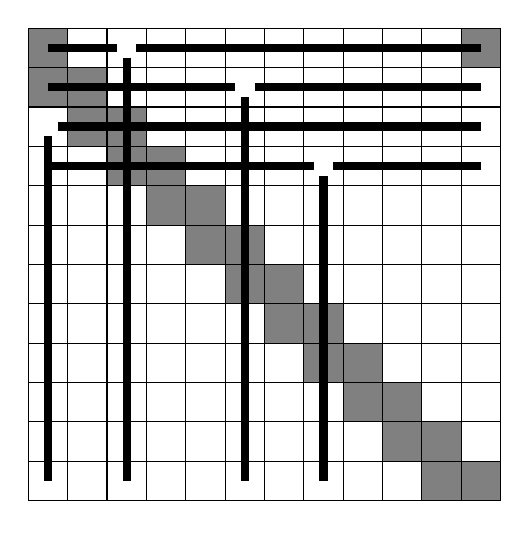
\begin{tikzpicture}[scale = 0.5]
    \path (0,-0.5) -- (0,6.5);
    \foreach \i in {0,...,11} { \fill[gray] (\i, 12-\i) rectangle (\i + 1, 11 - \i); }
    \foreach \i in {0,...,10} { \fill[gray] (\i, 11-\i) rectangle (\i + 1, 10 - \i); }
    \fill[gray] (11,11) rectangle (12,12);
    \draw (0,0) grid (12,12);
    \node (R1) at (2.5, 11.5) {\Large\symrook};
    \node (R2) at (5.5, 10.5) {\Large\symrook};
    \node (R3) at (0.5, 9.5) {\Large\symrook};
    \node (R4) at (7.5, 8.5) {\Large\symrook};
    \draw[line width = 3]
      (0.5,11.5) -- (R1) -- (11.5,11.5)
      (R1) -- (2.5,0.5)
    ;
    \draw[line width = 3]
      (0.5,10.5) -- (R2) -- (11.5,10.5)
      (R2) -- (5.5,0.5)
    ;
    \draw[line width = 3]
      (R3) -- (11.5,9.5)
      (R3) -- (0.5,0.5)
    ;
    \draw[line width = 3]
      (0.5,8.5) -- (R4) -- (11.5,8.5)
      (R4) -- (7.5,0.5)
    ;
  \end{tikzpicture}
  ~~~
  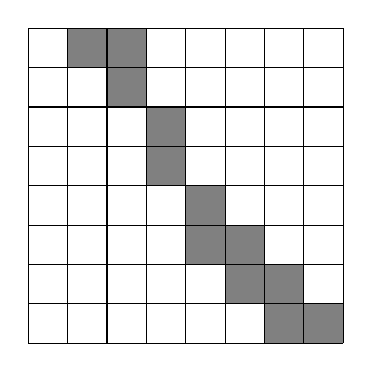
\begin{tikzpicture}[scale = 0.5]
    \path (0,-0.5) -- (0,6.5);
    \foreach \i/\j in {1/7, 2/6, 2/7, 3/4, 3/5, 4/2, 4/3, 5/2, 5/1, 6/1, 6/0, 7/0} {
      \fill[gray] (\i, \j) rectangle (\i + 1, \j + 1);
    }
    \draw (0,0) grid (8,8);
  \end{tikzpicture}
  ~~~
  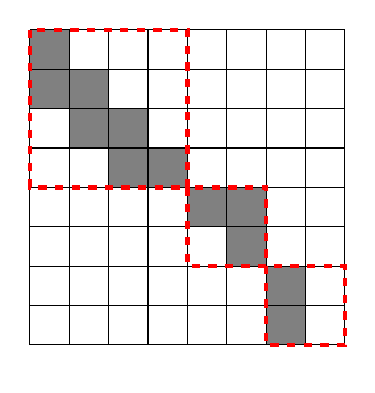
\begin{tikzpicture}[scale = 0.5]
    \path (0,-0.5) -- (0,6.5);
    \foreach \i/\j in {0/7, 0/6, 1/6, 1/5, 2/5, 2/4, 3/4, 4/3, 5/3, 5/2, 6/1, 6/0} {
      \fill[gray] (\i, \j) rectangle (\i + 1, \j + 1);
    }
    \draw (0,0) grid (8,8);
    \draw[ultra thick, dashed, red]
      (0,8) rectangle (4,4)
      (4,4) rectangle (6,2)
      (6,2) rectangle (8,0)
    ;
  \end{tikzpicture}
  \caption{
    xxx
  }
  \label{fig:partitionFromPrefix}
\end{figure}


\subsection{Complementary polynomials to m\'enage permutations with a given prefix}
Recap: We've taken a prefix, used it to find contiguous regions, used these to
find disjoint sub-boards related to $B_\alpha^c$, whose rook polynomials we know.
Now it's time to take these to count our number of m\'enage permutations with
the aforementioned prefix.
\begin{lemma}
  Given a board $B_\alpha^c$ that is partitioned into disjoint boards
  $b_1, b_2, \dots, b_m$, the rook polynomial of $B_\alpha^c$ is \[
    p_{B_\alpha^c}(x) = \prod_{i = 1}^m F_{b_i}(x).
  \]
\end{lemma}
\begin{proof}
  This follows directly from Lemma (TODO: rook polynomials of blocks)
  and Lemma (TODO: product of blocks is whole thing).
\end{proof}

Now that we know $p_{B_\alpha^c}$, we can use Lemma
(TODO: Complementary to original) to determine how many
m\'enage permutations there are with a given prefix. Because of Lemma
(TODO: all we need is the prefix to unrank), we have an algorithm to unrank.

\begin{example}
  Illustrating this particular example is too big to be of much interest, so
  here's a smaller example. There are $A000179(8) = 4738$ m\'enage
  permutations on $8$ letters. We'll use this algorithm to find the one
  at index $1000$.
  \begin{table}
    \center
    \begin{tabular}{|l|r|l|c|l|}
      \hline
      $\alpha$ & $\#\operatorname{prefix}(\alpha)$ & index range & composition & $\operatorname{unrank}_{i}(\alpha, \ell)$\\ \hline
      $1       $ & $0$   & $(0,0]$            & $-$       & $\operatorname{unrank}_{1000}(1,0)$          \\
      $2       $ & $787$ & $(0,787]$          & $(1,11)$  & $\operatorname{unrank}_{1000}(2,0)$          \\
      $3       $ & $791$ & $(787, 1578]$      & $(3,9)$   & $\operatorname{unrank}_{1000}(3,787)$        \\ \hline
      $31      $ & $0$   & $(787, 787]$       & $-$       & $\operatorname{unrank}_{1000}(31,787)$       \\
      $32      $ & $0$   & $(787, 787]$       & $-$       & $\operatorname{unrank}_{1000}(32,787)$       \\
      $33      $ & $0$   & $(787, 787]$       & $-$       & $\operatorname{unrank}_{1000}(33,787)$       \\
      $34      $ & $159$ & $(787, 946]$       & $(1,7)$   & $\operatorname{unrank}_{1000}(34,787)$       \\
      $35      $ & $166$ & $(946, 1112]$      & $(1,2,5)$ & $\operatorname{unrank}_{1000}(35,946)$       \\ \hline
      $351     $ & $24$  & $(946, 970]$       & $(0,2,5)$ & $\operatorname{unrank}_{1000}(351,946)$      \\
      $\cdots$   & $0$   & $(970,970]$        & $-$       & \\
      $354     $ & $34$  & $(970, 1004]$      & $(0,5)$   & $\operatorname{unrank}_{1000}(354,970)$      \\ \hline
      $3541    $ & $5$   & $(970,975]$        & $(0,5)$   & $\operatorname{unrank}_{1000}(3541,970)$     \\
      $3542    $ & $5$   & $(975,980]$        & $(0,5)$   & $\operatorname{unrank}_{1000}(3542,975)$     \\
      $\cdots$   & $0$   & $(980,980]$        & $-$       & \\
      $3546    $ & $8$   & $(980,988]$        & $(0,3)$   & $\operatorname{unrank}_{1000}(3546,980)$     \\
      $3547    $ & $10$  & $(988,998]$        & $(0,2,1)$ & $\operatorname{unrank}_{1000}(3547,988)$     \\
      $3548    $ & $6$   & $(998,1004]$       & $(0,4)$   & $\operatorname{unrank}_{1000}(3548,998)$     \\ \hline
      $35481   $ & $1$   & $(998,999]$        & $(0,4)$   & $\operatorname{unrank}_{1000}(35481,998)$    \\
      $35482   $ & $1$   & $(999,1000]$       & $(0,4)$   & $\operatorname{unrank}_{1000}(35482,999)$    \\ \hline
      $354821  $ & $0$   & $(999,999]$        & $(3)$     & $\operatorname{unrank}_{1000}(354821,999)$   \\
      $\cdots$   & $0$   & $(999,999]$        & $-$       & \\
      $354827  $ & $1$   & $(999,1000]$       & $(0,1)$   & $\operatorname{unrank}_{1000}(354827,999)$   \\ \hline
      $3548271 $ & $1$   & $(999,1000]$       & $(0)$     & $\operatorname{unrank}_{1000}(3548271,999)$  \\ \hline
      $35482716$ & $1$   & $(999,1000]$       & $()$      & $\operatorname{unrank}_{1000}(35482716,999)$ \\ \hline
    \end{tabular}
    \caption[Steps for computing the $1000$th m\'enage permutation in $S_8$.]{
      The recursive computation of the 1000th m\'enage permutation.
    }
  \end{table}
\end{example}

\section{Generalizations and Open Questions}
\subsection{Other restricted permutations}
Doron Zeilberger considers a more general family of restricted permutations.
\begin{definition}[\cite{Zeilberger2014}]
  Let $S \subset \mathbb Z$, then a \textit{$S$-avoiding permutation} is a
  permutation $\pi \in S_n$ such that \[
    \pi(i) - i - s \not\equiv 0 \bmod n \text{ for all } i \in [n] \text{ and } s \in S.
  \]
\end{definition}

\begin{example}
  Ordinary permutations are $\emptyset$-avoiding permutations,
  derangements are $\{0\}$-avoiding permutations, and
  we've defined menag\'e permutations as $\{-1,0\}$-avoiding permutations.

  The results in this paper generalize pretty easily to $\{i,i+1\}$-avoiding
  permutations for all $i$.
\end{example}

\subsection{Observation about Lyndon Words after? a given prefix}
\begin{definition}
  A \textit{Lyndon word} is a string that is the unique minimum with respect
  to all of its rotations.
\end{definition}
\begin{example}
  $00101$ is a Lyndon word because
  $00101 = \min\{00101, 01010, 10100, 01001, 10010\}$ is the unique minimum of
  all of its rotations.

  $011011$ is not a Lyndon word because while $011011 = \min\{011011, 110110, 101101, 011011, 110110, 101101\}$,
  it is not the \textbf{unique} minimum.
\end{example}
\begin{conjecture}
  Let $\mathcal{E}^{-1}$ denote the inverse Euler transform.
  Then the number of length $n+1$ Lyndon words that start with a prefix
  $\alpha$ follows a ``simple'' linear recurrence for sufficiently large $n$.
\end{conjecture}


% Using single-space for reference list.
\begin{singlespace}
% Bibliography
\phantomsection
\addcontentsline{toc}{chapter}{References}%
\markboth{References}{References}%
\printbibliography[title=References]
\end{singlespace}

% Appendices
\setcounter{section}{0} % Work around for weird Appendix numbering.
\phantomsection
\addcontentsline{toc}{chapter}{Appendices}%
\markboth{Appendices}{Appendices}%
\chapter*{Appendices}
\renewcommand\thesection{\Alph{section}}
\renewcommand*{\thesubsection}{\Alph{section}.\arabic{subsection}}
\begingroup
\numberwithin{equation}{section}
% Appendix source files
\section{An algorithm for unranking m\'enage permutations}
\label{apndx:haskell}
In this section, we will provide Haskell implementations of the functions in
Section \ref{cha:UnrankingMenage}. Each section of code will reference its
precedent in that section. We start by importing some relevant libraries
some naming conventions.

\begin{singlespace}\begin{verbatim}
import Data.List (sort, nub, intersect)

type Prefix = [Int]
type Coefficients = [Integer]
type PrefixCount = Prefix -> Integer
\end{verbatim}\end{singlespace}

\subsection{Unranking from prefix counts}

We begin with the function \texttt{unrank}, which implements
$\operatorname{unrank}_\mathcal{C}(i)$, as shown in Lemma
\ref{lemma:unrankFromPrefix}. The internal function
\texttt{recurse} corresponds to the recursive function $f_i^\mathcal{C}$.
\begin{singlespace}\begin{verbatim}
unrank :: Int ->                 -- Alphabet of n letters
          Int ->                 -- Words of length k
          (Prefix -> Integer) -> -- #prefix function
          Integer ->             -- Unrank at i
          Prefix                 -- Word at rank i
unrank n k prefixCounter i = recurse (0, 0) 1 [] where
  recurse :: (Integer, Integer) -> -- index range for prefix (a, b]
              Int ->                -- candidate for current letter
              Prefix ->             -- established prefix
              Prefix                -- word at index
  recurse (a, b) c prefix
    | c > n              = error "Out of range!"
    | length prefix == k = prefix
    | a < i && i <= b    = recurse (a, b') 1 (prefix  ++ [c])
    | otherwise          = recurse (b, b'') (c + 1) prefix where
    b'      = a + prefixCounter (prefix ++ [c, 1])
    b''     = b + prefixCounter (prefix  ++ [c + 1])
\end{verbatim}\end{singlespace}

\subsection{Counting derangements with prefixes}
This part of the code contains three functions, each of them take a parameter
$n$, which indicates the number of letters in the derangement.
The first function, \texttt{invalidDerangementPrefix}, also takes a prefix
$\alpha$ and checks to see if it includes duplicate values or has
letters in forbidden positions.
The function \texttt{derangementPrefixCount}
is equivalent to the function $\#\operatorname{prefix}_\mathcal{D}$,
as described in Corollary \ref{cor:derangementsWithPrefix}.
The function \texttt{unrankDerangement} is equivalent to the function
$\operatorname{unrank}_\mathcal{D}$ as described in
Lemma \ref{lemma:unrankFromPrefix}.
\begin{singlespace}\begin{verbatim}
invalidDerangementPrefix :: Int -> Prefix -> Bool
invalidDerangementPrefix _ prefix = containsDupes || invalidPosition where
  containsDupes = prefix /= (nub prefix)
  invalidPosition = any (id) $ zipWith (==) [1..] prefix

derangementPrefixCount :: Int -> Prefix -> Integer
derangementPrefixCount n prefix
  | invalidDerangementPrefix n prefix = 0
  | otherwise = sum $ map (\j -> term j) [0..squareCount] where
    k = length prefix
    squareCount = fromIntegral $ n - k - length (intersect [k+1..n] prefix)
    n' = fromIntegral n
    k' = fromIntegral k
    term j = (-1)^j * binomial squareCount j * factorial (n' - k' - j)

unrankDerangement :: Int -> Integer -> Prefix
unrankDerangement n = unrank n n (derangementPrefixCount n)
\end{verbatim}\end{singlespace}

\subsection{Decompose complementary m\'enage}
These next two function decompose a derived complementary board into
staircase-shaped blocks.
The first function, \texttt{getColGroups}, corresponds to the partition
into contiguous parts refered to in Lemma \ref{lem:subBoardSizes}.
The second function, \texttt{blockSizesFromPrefix} goes on to implement the
sum in this lemma.
\begin{singlespace}\begin{verbatim}
getColGroups :: Int -> Prefix -> [[Int]]
getColGroups n prefix = filter (not . null) $ colGroups where
  cols = 0 : (sort prefix) ++ [n+1]
  colGroups = zipWith (\a b ->  [a+1..b-1]) cols (tail cols)

blockSizesFromPrefix :: Int -> Prefix -> [Int]
blockSizesFromPrefix n prefix = map (sum . map colCells) colGroups where
  colGroups = getColGroups n prefix
  k = length prefix
  colCells c
    | c < k      = 0
    | c == k     = 1
    | c == n     = 1
    | otherwise  = 2
\end{verbatim}\end{singlespace}

\subsection{Complementary polynomials}
Since the functions above compute the size of the boards staircase-shaped
sub-boards, the can hand these values to \texttt{fibonacciPoly}, which
implements Fibonacci polynomials as described in
Definition \ref{def:FibonacciPolynomial}. These match the rook polynomials of
the disjoint staircase-shaped sub-boards, so in
\texttt{complementaryRookPolynomial}, the appropriate polynomials are multiplied
together and the coefficients are extracted to implement
Lemma \ref{lemma:CountsFromComplementaryPolynomials}.
\begin{singlespace}\begin{verbatim}
fibonacciPoly :: Int -> Coefficients
fibonacciPoly = (!!) fibonacciPolynomials where
  fibonacciPolynomials = [1] : [1] : recurse [1] [1] where
    recurse f g = h : recurse g h where
      h = ([0,1] .*. f) .+. g

complementaryRookPolynomial :: Int -> Prefix -> Coefficients
complementaryRookPolynomial n prefix = foldr (.*.) [1] blockPolys where
  blockPolys = map (\i -> fibonacciPoly (i + 1)) blockSizes where
    blockSizes = blockSizesFromPrefix n prefix
\end{verbatim}\end{singlespace}

\subsection{Putting it together}
This part of the code contains three functions, each of them take a parameter
$n$, which indicates the number of letters in the m\'enage permutation.
The first function, \texttt{invalidMenagePrefix}, also takes a prefix
$\alpha$ and checks to see if it includes duplicate values or has
letters in forbidden positions.
The function \texttt{menagePrefixCount}
is equivalent to the function $\#\operatorname{prefix}_\pazocal{M}$,
as described in Corollary \ref{cor:derangementsWithPrefix}.
The function \texttt{unrankDerangement} is equivalent to the function
$\operatorname{unrank}_\pazocal{M}$ as described in
Lemma \ref{lemma:unrankFromPrefix}.
\begin{singlespace}\begin{verbatim}
invalidMenagePrefix :: Int -> Prefix -> Bool
invalidMenagePrefix n prefix = containsDuplicates || invalidPosition where
  containsDuplicates = prefix /= (nub prefix)
  invalidPosition = any inRestrictedPosition $ zip [0..] prefix where
    inRestrictedPosition (i, x) = (x `mod` n == i) || (x == i + 1)

menagePrefixCount :: Int -> Prefix -> Integer
menagePrefixCount n prefix
  | invalidMenagePrefix n prefix = 0
  | otherwise      = recurse 0 crp where
  n' = fromIntegral (n - length prefix)
  crp = complementaryRookPolynomial n prefix
  recurse k (c:cs) = (-1)^k * c * factorial (n'-k) + recurse (k+1) cs
  recurse _ [] = 0

unrankMenage :: Int -> Integer -> Prefix
unrankMenage n = unrank n n (menagePrefixCount n)
\end{verbatim}\end{singlespace}

\subsection{Miscellanea}
These are helper functions that are needed to be included in order for the
code to compile. The first two functions add and multiply list representations
of polynomials, and the third and fourth function implement the factorial
function and the binomial coefficient.
\begin{singlespace}\begin{verbatim}
-- The polynomial a + bx + cx^2 ... is represented as
-- [a, b, c, ...]
-- These are helper functions for adding and multiplying polynomials
(.+.) :: Coefficients -> Coefficients -> Coefficients
(.+.) p1 [] = p1
(.+.) [] p2 = p2
(.+.) (a:p1) (b:p2) = (a + b) : (p1 .+. p2)

(.*.) :: Coefficients -> Coefficients -> Coefficients
(.*.) p1 [] = []
(.*.) [] p2 = []
(.*.) p1 p2 = foldr1 (.+.) termwiseProduct where
  termwiseProduct = map f $ zip [0..] p1 where
    f (i, x) = replicate i 0 ++ map (*x) p2

factorial :: Integer -> Integer
factorial n = factorial' n 1 where
  factorial' 0 accum = accum
  factorial' n accum = factorial' (n - 1) (accum * n)

binomial :: Integer -> Integer -> Integer
binomial _ 0 = 1
binomial 0 _ = 0
binomial n k
  | n < k'    = 0
  | otherwise = product [k' + 1..n] `div` factorial (n - k') where
    k' = max k (n - k)
\end{verbatim}\end{singlespace}

\section{Unranking combinatorial objects}
\label{apndx:unranking}
\subsection{Compositions}
\begin{definition}
  A \textbf{composition} of $n \in \mathbb{N}_{>0}$ is a sequence of
  strictly positive integers summing to $n$. We denote the set of compositions
  of n by $\pazocal C_n$.
\end{definition}

\begin{lemma}[\cite{Stanley2011EC1}] % (p. 18)
  The number of compositions of $n$ is $\#\pazocal C_n = 2^{n-1}$.
\end{lemma}

\begin{proposition}
  If $\alpha$ is a sequence of positive integers such that
  $\operatorname{sum}(\alpha) \leq n$, then
  the number of compositions of $n$ that start with the prefix $\alpha$
  is \begin{equation}
    \#\operatorname{prefix}_{\pazocal{C}_n}(\alpha) = \begin{cases}
      1 & \alpha \in \pazocal{C}_n \\
      2^{n - \operatorname{sum}(\alpha) - 1} & \text{otherwise}.
    \end{cases}
  \end{equation}
\end{proposition}

\begin{definition}
  For $k > 0$, a $k$\textbf{-composition} of $n \in \mathbb{N}_{>0}$
  is a sequence of length $k$ consisting of strictly positive integers that sum
  to $n$. We denote the set of $k$-compositions of $n$ by $\pazocal C_n^{k}$.
\end{definition}

\begin{lemma}[\cite{Stanley2011EC1}]
  The number of $k$-compositions of $n$ is $\#\pazocal C_n^{k} = \binom{n-1}{k-1}$.
\end{lemma}

\begin{proposition}
  If $\alpha \in \pazocal{C}_n^{k}$ or if $\alpha$ is
  a sequence of positive integers of length $\ell < k$ such that
  ${\operatorname{sum}(\alpha) < n}$ or
  then the number of $k$-compositions of $n$ that start with the prefix $\alpha$
  is \begin{equation}
    \#\operatorname{prefix}_{\pazocal{C}_n}(\alpha) = \begin{cases}
      1 & \alpha \in \pazocal{C}_n^{k} \\
      \binom{n - \operatorname{sum}(\alpha) - 1}{k - \ell - 1} & \text{otherwise}.
    \end{cases}
  \end{equation}
\end{proposition}

\subsection{Partitions}
\begin{definition}
  A \textbf{partition} of $n \in \mathbb{N}_{>0}$ is a weakly decreasing
  sequence of strictly positive integers summing to $n$. We denote the set of
  partitions of $n$ by $\pazocal P_n$.

  The set of partitions of $n$ with largest part at most
  $j$ is denoted $\pazocal P_n^{\leq j}$.
\end{definition}

\begin{lemma}[\cite{Stanley2011EC1}]
  The ordinary generating for the number of partitions of $n$ is \begin{equation}
    \sum_{i=0}^\infty \#\pazocal P_n q^n = \prod_{i=1}^\infty \frac{1}{1-q^j},
  \end{equation}
  and the ordinary generating for the number of partitions of $n$ with largest part
  as most $j$ is \begin{equation}
    \sum_{i=0}^\infty \#\pazocal P_n^{\leq j} q^n = \prod_{i=1}^k \frac{1}{1-q^j}.
  \end{equation}
\end{lemma}

\begin{proposition}
  If either $\alpha \in \pazocal{P}_n$ or $\alpha$ is
  a decreasing sequence of positive integers such that
  ${\operatorname{sum}(\alpha) < n}$ or
  then the number of partitions of $n$ that start with the prefix $\alpha$
  is \begin{equation}
    \#\operatorname{prefix}_{\pazocal{P}_n}(\alpha) = \begin{cases}
      1 & \alpha \in \pazocal{C}_n^{k} \\
      \#\pazocal P_{n-\operatorname{sum}(\alpha)}^{\leq \operatorname{min}(\alpha)} & \text{otherwise}.
    \end{cases}
  \end{equation}
\end{proposition}

\endgroup

\end{document}
